%!TEX root = ../thesis.tex
%*******************************************************************************
%*********************************** Sixth Chapter *****************************
%*******************************************************************************
\cleardoublepage
\chapter{Rare event estimation using Bernstein adaptive nonparametric sampling}
\label{chpt:6}
%*******************************************************************************
\hfill
\localtableofcontents
\newpage

\begin{tcolorbox}[colback=gray!5!white, colframe=gray!5!white, coltitle=gray, coltext=gray, fontupper=\footnotesize, fontlower=\footnotesize, title=\textbf{Parts of this chapter are adapted from the following publication:}]
    \begin{itemize}
        \item[\ding{125}] E. Fekhari, V. Chabridon, J. Muré and B. Iooss (2023). ``Bernstein adaptive nonparametric conditional sampling: a new method for rare event probability estimation''. In: \textit{Proceedings of the 14th International Conference on Applications of Statistics and Probability in Civil Engineering (ICASP14)}.
        \item[\ding{43}] This work was rewarded by the ``CERRA\footnotemark~Student Recognition Award'' at the ICASP14 conference.
    \end{itemize}
\end{tcolorbox}

\footnotetext{CERRA stands for ``international Civil Engineering Risk and Reliability Association''.}

%============================================================%
%============================================================%
\section{Introduction}
%============================================================%
%============================================================%

Assessing the reliability of systems such as offshore wind turbines, often involves the estimation of rare event probabilities. 
In the reliability analysis framework introduced in Section~\ref{sec:reliability}, the performance of a system is typically modeled by a deterministic scalar function, denoted by $g: \iD_\bx \subseteq \R^d \rightarrow \R$, and referred to as the \textit{limit-state function} (LSF). 
A critical threshold on the system's output, denoted by $\yth \in \R$, enables to define the \textit{failure domain} as $\iF = \{\bx \in \iD_\bx \, | \,  g(\bx) \leq \yth\}$. 
Considering a probabilistic framework, the uncertain inputs are modeled by a continuous random vector $\bX \in \iD_\bx$ distributed according to a PDF $f_\bX$. 
In this scenario, uncertainty propagation consists in composing the random vector $\bX$ with the function $g$ to obtain the output variable of interest $Y = g(\bX) \in \R$. 
Then, a common risk measure in reliability analysis is the \textit{failure probability} \citep{rockafellar_2015}, denoted by $\pf$, representing the probability of the system crossing the threshold $\yth$:
\begin{equation}
    \label{eq:failure_proba_c6}
    \pf = \P(g(\bX) \leq \yth)
        = \int_{\iD_\bx} \1_\{\iF\}(\bx) f_\bX(\bx) \, \dd\bx.
\end{equation}
The usual convention presented in Section~\ref{sec:reliability} allows to modify the LSF in order to set the threshold to zero. 
Moreover, as presented previously, the main methods for rare event estimation can be divided into two groups \citep{MorioBalesdent2015}: 
\textit{(i)} first the geometric approaches, such as the first-/second-order reliability method (FORM/SORM) whose aim is to approximate the LSF by a first-/second-order Taylor expansion at the most probable failure point; 
\textit{(ii)} second the simulation-based techniques such as the crude Monte Carlo method and many other variance reduction techniques. 
Unfortunately, FORM/SORM methods do not provide much statistical information as they are purely geometric approaches. 
Meanwhile, estimating a rare event probability by crude Monte Carlo becomes rapidly intractable for engineering applications. 
To overcome this limit, advanced simulation techniques have been developed: among others, one can mention several variance reduction methods such as the nonadaptive and adaptive versions of the importance sampling \citep{RubinsteinKroese1981} and splitting techniques \citep{cerou2012sequential} such as subset simulation (SS) \citep{AuBeck2001}.

In SS, the idea is to write the rare event probability $\pf$ as a product of larger conditional probabilities, each one of them being easier to estimate. 
To generate intermediary conditional samples, this method uses Markov chain Monte Carlo (MCMC) sampling, which presents a large panel of dedicated algorithms \citep{Papaioannou_PEM_2015}. 
However, MCMC algorithms are known to be highly tunable algorithms and to produce non-i.i.d. samples, which consequently, cannot always be used for direct unbiased statistical estimation (e.g., for $\pf$ but also for sensitivity indices). 

Adaptive importance sampling infers conditional distributions before using an importance sampling estimator of the failure probability. 
The set of auxiliary distributions converging towards the failure domain is either fitted by parametric approaches (e.g., using the cross-entropy method \citealp{rubinstein_2004_CE}), or nonparametric methods (e.g., using multivariate KDE \citealp{zhang_1996_NIS, Morio_RESS_2011}). 
The main drawback of cross-entropy adaptive importance sampling (CE-AIS) is its limited flexibility, which makes it perform badly in the case of multimodal failure domains. 
Meanwhile, nonparametric adaptive importance sampling (NAIS) inherits its drawbacks from the multivariate KDE (i.e., significant performance drop for medium to high dimension). 
The limitations associated with these two classes of IS have been addressed by several authors \citep{kurtz_song_2013_aisce,papaioannou_2016, geyer_2019_aisce, uribe_2021_aisce}.

The present work proposes a new rare event estimation method, ``Bernstein adaptive nonparametric conditional sampling'' (\abv{bancs}), adopting the same adaptive importance sampling structure as CE-AIS or NAIS while using a different mechanism to fit conditional distributions. 
This algorithm decomposes the fit of the intermediary conditional distributions into two steps: a fit of their marginals by univariate KDE, and a fit of their copula with the \emph{empirical Bernstein copula} (abbreviated EBC and introduced in Section~\ref{sec:nonparametric_copula}). 
Compared to direct multivariate KDE in NAIS, this decomposition should simplify the inference in medium to high dimension. 
Additionally, unlike SS, the proposed method generates i.i.d. samples of the intermediary conditional distributions. 
In practice, such i.i.d. samples may also be used to estimate dedicated reliability-oriented sensitivity indices (see e.g., \citealp{chabridon2021global,marrel_chabridon_2021}). 
To do so, the present chapter introduces kernel-based reliability-oriented sensitivity indices and their direct estimation as a post-processing of the BANCS algorithm. 

In this chapter, Section~\ref{sec:bancs} will introduce the BANCS algorithm for rare event estimation. 
Then, Section~\ref{sec:bancs_bench} will apply this method to three test cases and analyze the results w.r.t. NAIS and SS performances. 
Section~\ref{sec:bancs_rosa} will present a kernel-based reliability-oriented sensitivity index and illustrate its estimation on samples generated by the BANCS algorithm. 
Then, the last section present some conclusions and research perspectives.

%\elias{Terminology: elite set or elite sample can be used to describe the points that failed at each step}
\begin{remark}
    BANCS was initially proposed in \citet{fekhari_ICASP_2023}, using the failure probability estimator from the SS algorithm (see \eq{eq:pf_SS}). 
    Switching to an adaptive importance sampling estimator (see e.g., \eq{eq:pf_NAIS}) notably improved the method.    
\end{remark}



%============================================================%
%============================================================%
\section{Bernstein adaptive nonparametric conditional sampling (BANCS)}\label{sec:bancs}
%============================================================%
%============================================================%

The BANCS algorithm uses the same structure as other adaptive importance sampling methods (e.g., NAIS or CE-AIS introduced in Section~\ref{sec:reliability}) while employing a different approach to fit the intermediate conditional distributions. 
The proposed algorithm is described in Algorithm \ref{alg:bancs} at iteration $k$, after estimating the intermediary $p_0$-quantile $\widehat{q}_{[k]}^{\, p_0}$, a nonparametric model is fitted on the set $\mathbf{A}_{[k+1]}$ of all samples leading to values below $\widehat{q}_{[k]}^{\, p_0}$ (also called ``elite set'').  
This inference is done by coupling a set of marginals fitted by univariate KDE, with a copula fitted using the EBC. 
The generation of the next i.i.d. $N$-sized sample $\bX_{[k+1], N}$ from the conditional distributions is straightforward and does not require any MCMC sampling like in SS. 
Note that the BANCS method does not require any iso-probabilistic transform either.

%%%%%%%%%%%%%%%%%%%%%%%%%%%%%%%%%%%%%%%%%%%%%%%%%%%%%%%%%%%%%
\begin{algorithm}[h]
    \caption{Bernstein adaptive nonparametric conditional sampling (BANCS).}\label{alg:bancs}
    \footnotesize
    \begin{algorithmic}[1]
        \LeftComment{\textbf{Inputs:}}
        \State $f_\bX$: joint PDF of the inputs
        \State $g(\cdot)$: LSF
        \State $\yth \in \R$: threshold defining the failure event 
        \State $N$: number of samples per iteration
        \State $m \in \N$: parameter of the EBC fitting
        \State $p_0 \in ]0, 1[$: empirical quantile order (rarity parameter)
        \LeftComment{\textbf{Algorithm:}}
        \State Set $k = 0$ and $\what{f}_{[0]} = f_\bX$
        \State Sample $\bX_{[0], N} = \left\{\bx_{[0]}^{(i)}\right\}_{i=1}^N \overset{\text{i.i.d.}}{\sim} \what{f}_{[0]}$
        \State Evaluate $Y_{[0], N} = \left\{g(\bx_{[0]}^{(i)})\right\}_{i=1}^N$
        \State Estimate the empirical $p_0$-quantile $\widehat{q}_{[0]}^{\, p_0}$ of the set $Y_{[0], N}$
        
        \While{$\widehat{q}_{[k]}^{\, p_0} > \yth$}
        \State Compute IS weights $\left\{w_{[k]}^{(i)}\right\}_{i=1}^N = \left\{\frac{f_\bX(\bx_{[k]}^{(i)})}{\widehat{f}_{[k]}(\bx_{[k]}^{(i)})}\right\}_{j=1}^N$
        \State Build a weighted elite set $\mathbf{A}_{[k+1]}=\sum_{l=1}^{k} \sum_{i=1}^N w_{[k]}^{(j)} \, \1_{\left\{g(\bx_{[l]}^{(i)}) \leq \widehat{q}_{[k]} \right\}}\left(\bx_{[k]}^{(i)}\right)$
        \State Fit marginals of the set $\mathbf{A}_{[k+1]}$ by KDE $\left\{\widehat{F}_j\right\}_{j=1}^d$
        \State Fit the copula of the set $\mathbf{A}_{[k+1]}$ by EBC $B_\bm(C_n)$
        \State Build a CDF $\widehat{F}_{[k+1]}(\bx) = B_m(C_n)\left(\widehat{F}_1(x_1), \dots, \widehat{F}_d(x_d)\right)$
        \State Sample $\bX_{[k+1], N} = \left\{\bx_{[k+1]}^{(i)}\right\}_{i=1}^N \overset{\text{i.i.d.}}{\sim} \widehat{f}_{[k+1]}$
        \State Evaluate $Y_{[k+1], N} = \left\{g(\bx_{[k+1]}^{(i)})\right\}_{i=1}^N$
        \State Estimate the empirical $p_0$-quantile $\widehat{q}_{[k+1]}^{\, p_0}$ of $Y_{[k+1], N}$
\State Set $k = k+1$
\EndWhile
\State Set $k_\# = k$
%\State Estimate $\widehat{\pf} = (1 - p_0)^{k_\#} \cdot \frac{1}{N} \sum_{j=1}^N \1_{\{g(\bX_{[k_\#]}^{(j)}) \geq \yth  \}}(\bX_{[k_\#]^{(j)}}) $
\State Estimate $\widehat{\pf}^{\mathrm{BANCS}} = \frac1N \sum_{i=1}^N w_{[k_\#]}^{(i)} \, \1_{\left\{g(\bx_{[k_\#]}^{(i)}) \leq \yth \right\}}\left(\bx_{[k_\#]}^{(i)}\right)$
\State Estimate $\what{\var}\left(\widehat{\pf}^{\mathrm{BANCS}}\right) = \frac{1}{N-1} \left[\frac1N \sum_{i=1}^N \left(w_{[k_\#]}^{(i)}\right)^2 \, \1_{\left\{g(\bx_{[k_\#]}^{(i)}) \leq \yth \right\}}\left(\bx_{[k_\#]}^{(i)}\right) \, - \, \left(\widehat{\pf}^{\mathrm{BANCS}}\right)^2\right]$
\LeftComment{\textbf{Outputs:}}
\State $\widehat{\pf}^{\mathrm{BANCS}}$, estimate of $\pf$
\end{algorithmic}
\end{algorithm}
%%%%%%%%%%%%%%%%%%%%%%%%%%%%%%%%%%%%%%%%%%%%%%%%%%%%%%%%%%%%%
\begin{figure}[!ht]
    \centering
    \begin{subfigure}[b]{0.49\linewidth}
        \centering
        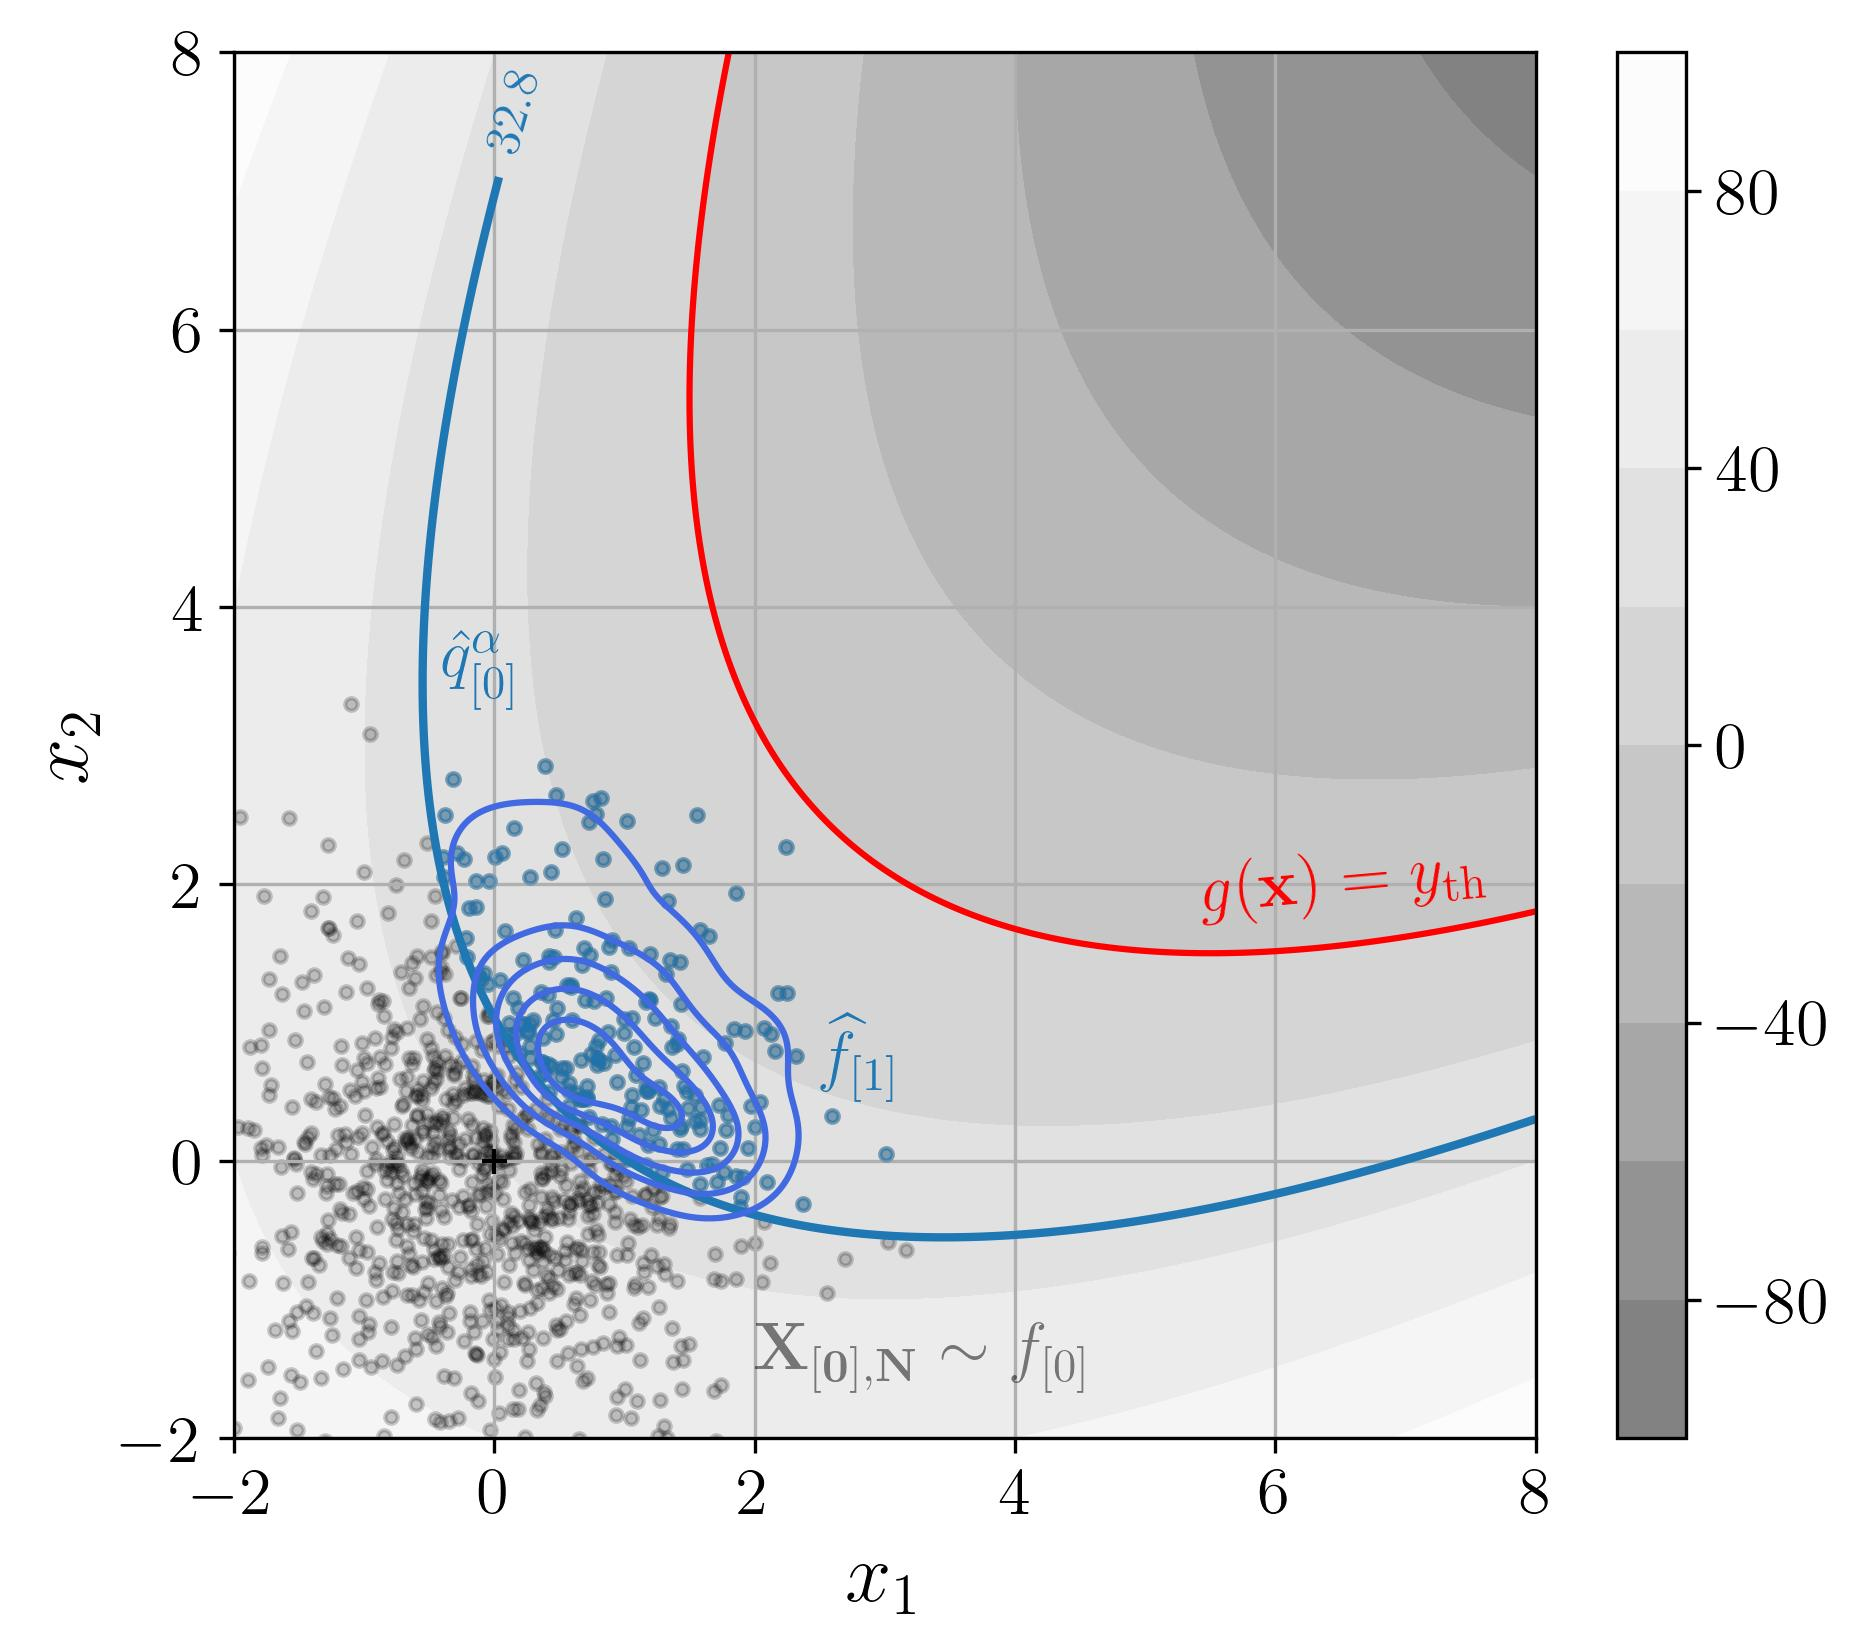
\includegraphics[width=\linewidth]{part3/figures/BANCS/bancs_illustration0.jpg}
        \caption{Iteration $k=0$.}
    \end{subfigure}
    \begin{subfigure}[b]{0.49\linewidth}
        \centering
        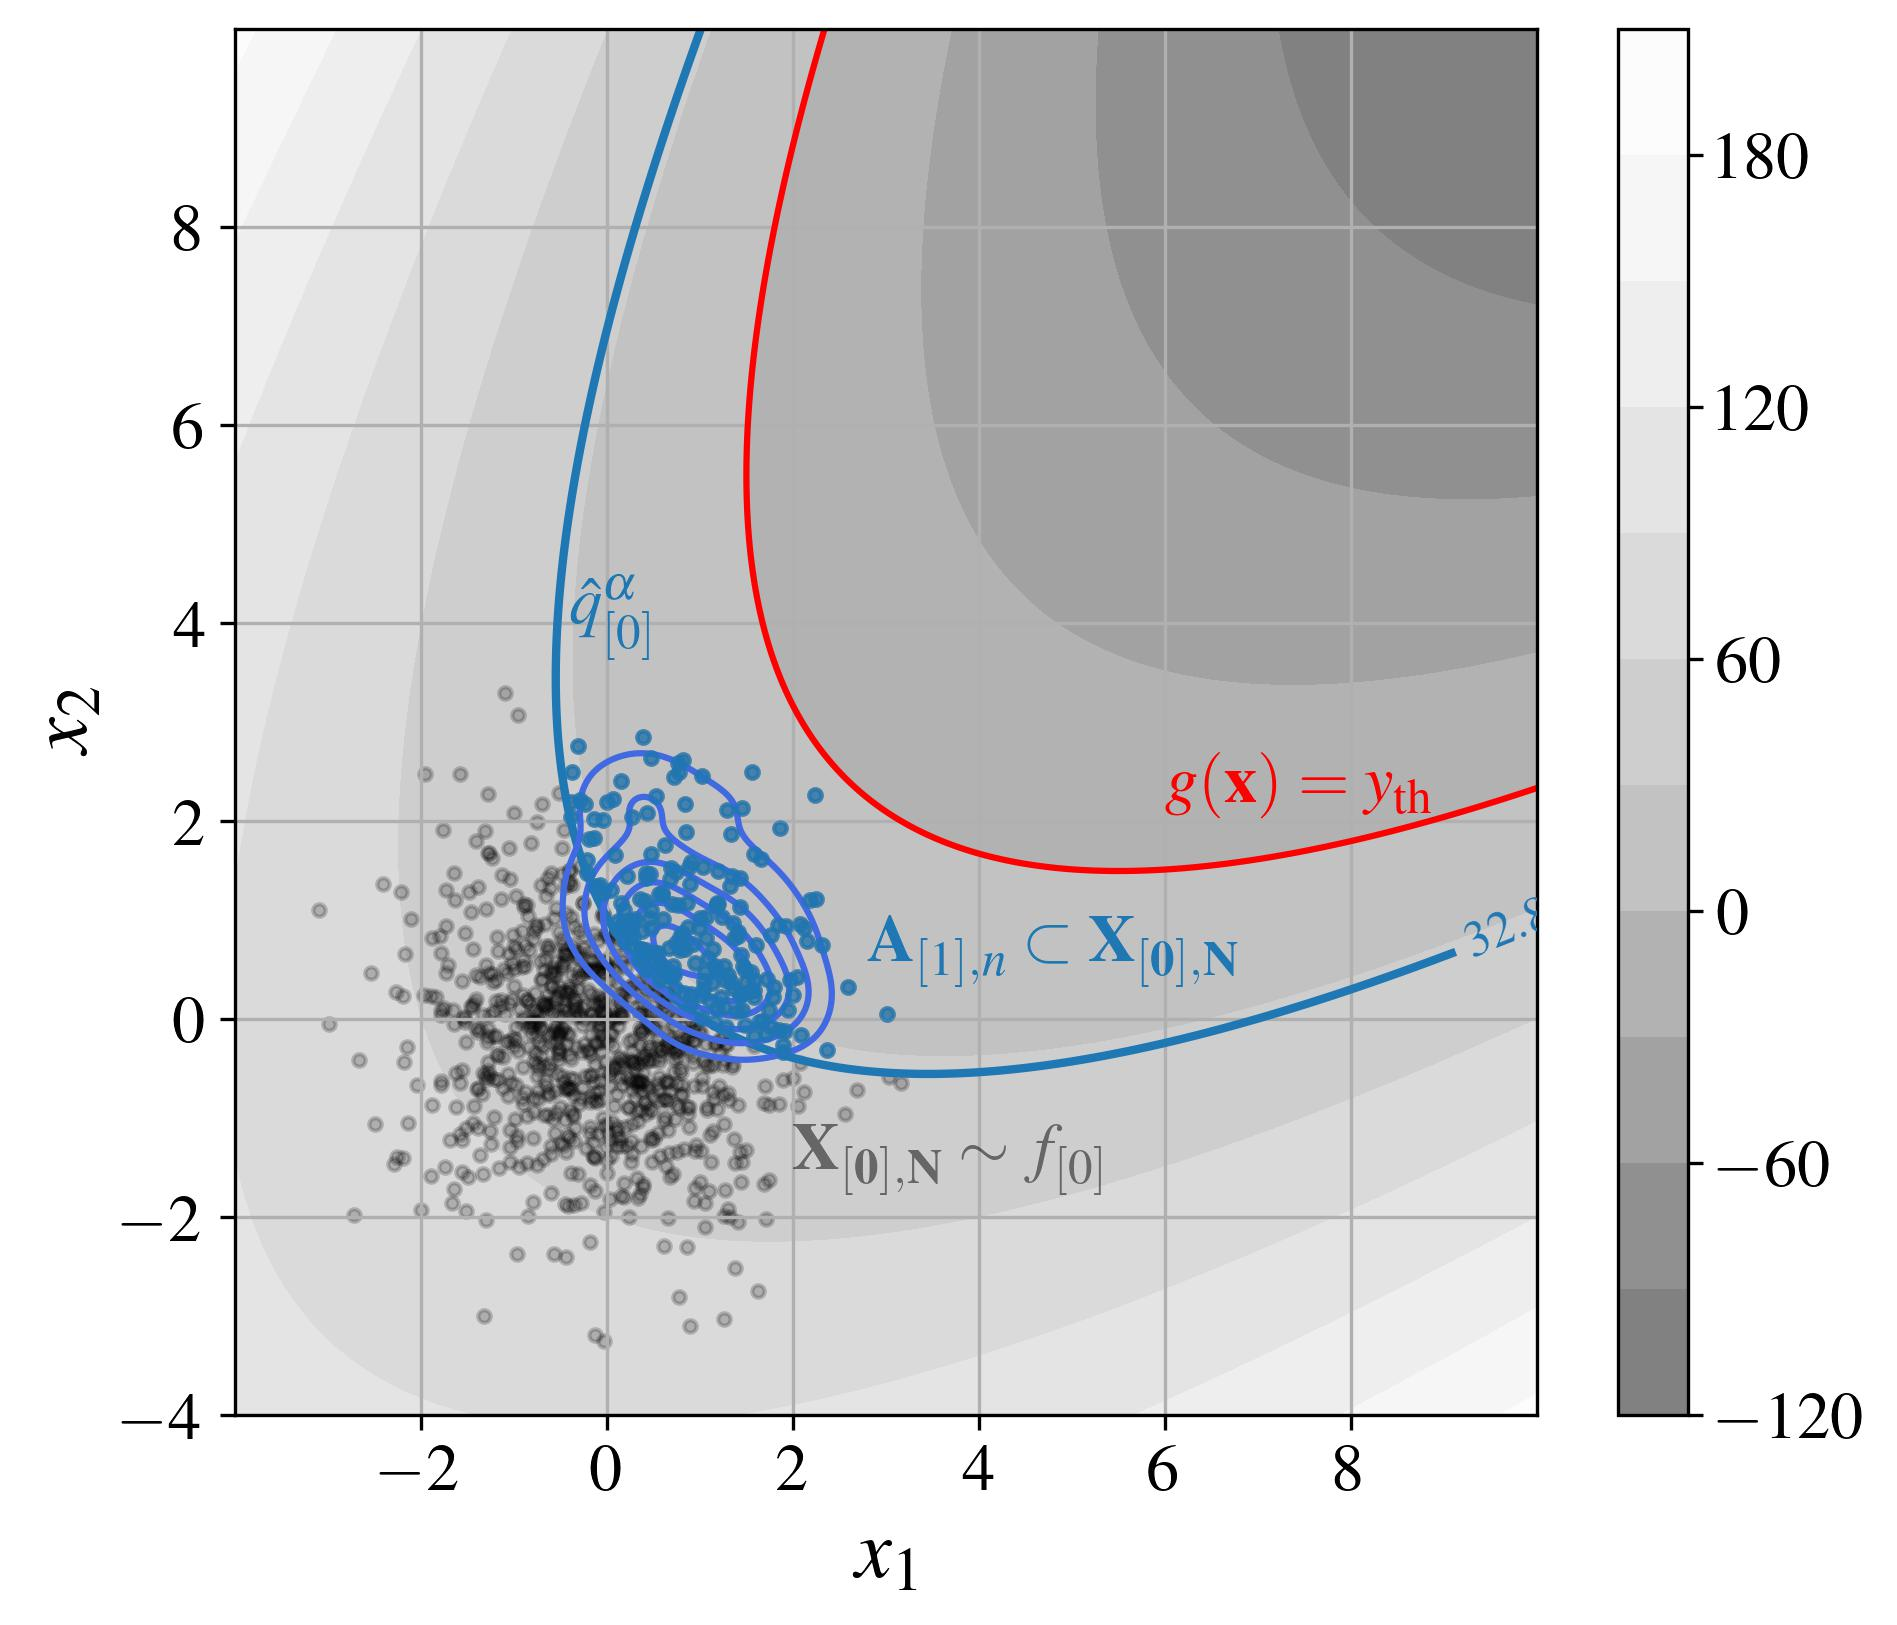
\includegraphics[width=\linewidth]{part3/figures/BANCS/bancs_illustration1.jpg}
        \caption{Iteration $k=1$.}
    \end{subfigure}
    \caption{BANCS algorithm applied to test case \#1: illustration of conditional sampling and nonparametric fit at the first and second iterations.}
    \label{fig:bancs_illustration}
\end{figure}
%%%%%%%%%%%%%%%%%%%%%%%%%%%%%%%%%%%%%%%%%%%%%%%%%%%%%%%%%%%%%

Nonparametric inference requires to tune the scaling parameters for KDE and the polynomial order $m$ (considered equal for all the input dimensions) for EBC. 
In the current implementation of BANCS, the KDE is tuned using Silverman's rule\footnotemark~\citep{silverman_1981} while the EBC is tuned to minimize an asymptotic mean integrated squared error (AMISE). 
As discussed in Chapter~\ref{chpt:3}, for a dataset with size $n$ and dimension $d$, the AMISE tuning for the EBC was defined by \citet{sancetta_satchell_2004} as:
\begin{equation}\label{eq:amise_tuning}
    m_{\mathrm{AIMSE}} = 1 + N^{2/(d+4)}
\end{equation}
In our experience, EBC tuning in \eq{eq:amise_tuning} works well for the BANCS algorithm and will be systematically used in the following. 
This tuning sets a rather low polynomial order to the EBC, which avoids overfitting issues. 
For small sample sizes (e.g., $N<100$), \citet{segers_2017} showed the limits of this tuning. 
However, the typical sample sizes used for rare event estimation should suit the AMISE tuning. 

\footnotetext{In the multivariate case, Silverman's rule is defined as follows: $\eta_{\mathrm{Silv.}} = \left(\frac1N \, \frac{4}{d+2}\right)^{1/(d+4)}$.}

Ultimately, the estimator of the probability from \eq{eq:failure_proba_c6} is written as a simple IS estimator on the last conditional distribution with PDF $\widehat{f}_{[k_\#]}$:
\begin{equation}
    \widehat{\pf}^{\mathrm{BANCS}} = \frac1N \sum_{i=1}^N \frac{f_\bX\left(\bx_{[k_\#]}^{(i)}\right)}{\widehat{f}_{[k_\#]}\left(\bx_{[k_\#]}^{(i)}\right)} \, \1_{\left\{g(\bx_{[k_\#]}^{(i)}) \leq \yth \right\}}\left(\bx_{[k_\#]}^{(i)}\right)\, , \quad \left\{\bx_{[k_\#]}^{(i)}\right\}_{i=1}^N  \overset{\text{i.i.d.}}{\sim} \widehat{f}_{[k_\#]} \, .
\end{equation}
This estimator also benefits from an IS variance, estimated using the same sample as previously:
\begin{equation}
    \what{\var}\left(\widehat{\pf}^{\mathrm{BANCS}}\right) = \frac{1}{N-1} \left[\frac1N \sum_{i=1}^N \left(\frac{f_\bX\left(\bx_{[k_\#]}^{(i)}\right)}{\widehat{f}_{[k_\#]}\left(\bx_{[k_\#]}^{(i)}\right)}\right)^2 \, \1_{\left\{g(\bx_{[k_\#]}^{(i)}) \leq \yth \right\}}\left(\bx_{[k_\#]}^{(i)}\right) \, - \, \left(\widehat{\pf}^{\mathrm{BANCS}}\right)^2\right]
\end{equation}

\fig{fig:bancs_illustration} illustrates the nonparametric fit and conditional sampling in the BANCS method on a two-dimensional reliability problem (later introduced as ``test case \#1'', see Subsection~\ref{sec:testcases}). 
At the iteration $k=0$, the conditional distribution fitted (with PDF represented by the blue isolines) slightly crosses the quantile border $\widehat{q}_{[0]}^{\, p_0}$ (in blue). 
Ideally, the conditional distribution fitted, with PDF denoted by $\what{f}_{[1]}$, should be bounded by this border. 
At the second iteration, the PDF of the conditional distribution denoted by $\what{f}_{[2]}$, is represented by the brown isolines. 
Unlike the inference of $\what{f}_{[1]}$, the fit of $\what{f}_{[2]}$ is realized on the samples from $\bX_{[1], N} \sim \what{f}_{[1]}$ and $\bX_{[0], N} \sim \what{f}_{[0]}$ which crossed the quantile $\widehat{q}_{[1]}^{\, p_0}$. 
Indeed, the samples $\bX_{[0], N} \sim \what{f}_{[0]}$ are weighted according to an IS procedure (see the lines 14 and 15 from Algorithm~\ref{alg:bancs}). 
Including the samples from the previous iterations refines the goodness-of-fit near the quantile border and significantly improves BANCS performances. 


%============================================================%
%============================================================%
\section{Numerical experiments}\label{sec:bancs_bench}
%============================================================%
%============================================================%
In the present section, the performances of BANCS algorithm are compared with the ones from SS and NAIS algorithms. 
The efficiency of SS depends on the choice and tuning of the MCMC algorithm \citep{Papaioannou_PEM_2015}. 
The proposed work uses the \ots implementation of the SS\footnote{SS: \url{https://openturns.github.io/openturns/latest/user_manual/_generated/openturns.SubsetSampling.html}}~(integrating a component-wise Metropolis-Hastings algorithm), 
and the \ots implementation of NAIS\footnote{NAIS: \url{https://openturns.github.io/openturns/latest/user_manual/_generated/openturns.NAIS.html}}.
An implementation of the BANCS method and the following numerical experiments are available in a public Git repository\footnote{BANCS: \url{https://github.com/efekhari27/bancs}}. 

In the following analytical numerical experiments, the intermediary probabilities were set to $p_0=0.1$ (following the recommendations from \citealp{AuBeck2001}), allowing a fair comparison with the usual SS implementation. 
The following intermediate sample sizes $N \in \{300, 500, 700, 1000, 2000, 5000, 10000\}$ are simulated.
Let us recall that the EBC tuning is set to minimize the AMISE, such that $m = 1 + N^{\frac{2}{d+4}}$. 
Finally, in order to take into account the variability of the method's results, each experiment is repeated 100 times, allowing the computation of a coefficient of variation $\widehat{\delta} = \frac{\sigma_{\widehat{\pf}}}{\mu_{\widehat{\pf}}}$. 
Since the SS estimator only provide an approximated value of its dispersion, an empirical estimation on repetitions is the most neutral way to compare the variability of several methods. 


%============================================================%
\subsection{Analytical test cases}\label{sec:testcases}
%============================================================%
The reference values of the failure probabilities associated with each problem studied hereafter are obtained by Monte Carlo estimation on very large samples (typically with size $N_{\mathrm{ref}} = 10^9$). 

%------------------------------------------------------------%
\paragraph{Test case \#1: Parabolic reliability problem.}
%------------------------------------------------------------%
This reliability problem, is defined by the function $g_1: \R^2 \rightarrow \R$:
\begin{equation}
    g_1(\bx)= (x_1 - x_2) ^ 2 - 8 \, (x_1 + x_2 - 5)\, ,
\end{equation}
with the input random vector $\bX = (X_1, X_2)$ following a standard 2-dimensional normal distribution. 
The reliability problem consists in evaluating: $p_{\mathrm{f}, 1} = \mathbb{P} ( g_1(\bX) \leq 0 ) = 1.31 \times 10^{-4}$.

%------------------------------------------------------------%
\paragraph{Test case \#2: Four-branch reliability problem.}
%------------------------------------------------------------%
This reliability problem (originally proposed by \cite{waarts2000structural}), is defined by the following function $g_2: \R^2 \rightarrow \R$:
\begin{align}
  g_2(\bx) = \min \begin{pmatrix}
    3+0.1 \, (x_1-x_2)^2-\frac{(x_1+x_2)}{\sqrt{2}}\\
    3+0.1\, (x_1-x_2)^2+\frac{(x_1+x_2)}{\sqrt{2}}\\
    (x_1-x_2)+ \frac{7}{\sqrt{2}}\\
    (x_2-x_1)+ \frac{7}{\sqrt{2}}
  \end{pmatrix}\, ,
\end{align}
with the input random vector $\bX = (X_1, X_2)$ following a standard 2-dimensional normal distribution. 
The reliability problem consists in evaluating: $p_{\mathrm{f}, 2} = \mathbb{P} ( g_2(\bX) \leq 0 ) =  2.22 \times 10^{-3}$.

%------------------------------------------------------------%
\paragraph{Test case \#3: Modified Ishigami reliability problem.}
%------------------------------------------------------------%
This reliability problem (inspired by \citealp{lemaitre_2015_PLI}), is defined by the following function $g_3: \R^3 \rightarrow \R$:
\begin{equation}
    g_3(\bx) = \sin(x_1) + 7 \, \sin(x_2)^2 + \frac{x_3^4 \, \sin(x_1)}{10} - 10.5.
\end{equation}
with the input random vector $\bX = (X_1, X_2, X_3)$ following a standard 3-dimensional normal distribution. 
The reliability problem consists in evaluating: $p_{\mathrm{f}, 3} = \mathbb{P} ( g_3(\bX) \leq 0 ) =  1.94 \times 10^{-5}$.

%------------------------------------------------------------%
\paragraph{Test case \#4: Medium-dimensional reliability problem.}
%------------------------------------------------------------%
This reliability problem (proposed by \citealp{yun2018efficient}), is defined by the following function $g_4 : \R^7 \rightarrow \R$:

\begin{equation}
    g_4(\bx) = 15.59 \times 10^4 - \frac{x_1 x_3^2}{2 x_3^2} \, \frac{x_2^4 - 4 x_5 x_6 x_7^2 + x_4 (x_6 + 4 x_5 + 2 x_6 x_7)}{x_4 x_5 (x_4 + x_6 + 2 x_6 x_7)}\, ,
\end{equation}
with the input random vector $\bX = (X_1, \dots, X_7)$, following a product of normal distributions defined in \cite{yun2018efficient}. 
The reliability problem consists in evaluating the probability: $p_{\mathrm{f}, 4} = \mathbb{P} ( g_4(\bX) \leq 0 ) =  8.10 \times 10^{-3}$.


%------------------------------------------------------------%
\paragraph{Test case \#5: Medium-dimensional nonlinear oscillator problem.}
%------------------------------------------------------------%
This reliability problem (initially introduced by \citealp{destefano_1990}), is defined by the following function $g_5 : \R^8 \rightarrow \R$:

\begin{equation}
    g_5(\bx) = F_s - 3 k_s \sqrt{\frac{\pi S_0}{4 \zeta_s \omega_s^3} \, \frac{\zeta_a \zeta_s}{\zeta_p \zeta_s (4 \zeta_a^2 + \theta^2) + \gamma \zeta_a^2} \, \frac{\omega_p \, (\zeta_p \omega_p^3 + \zeta_s \omega_s^3)}{4 \zeta_a \omega_a^4}} \, ,
\end{equation}
where $\bx = \left(m_p, m_s, k_p, k_s, \zeta_p, \zeta_s, F_s, S_0\right)$,  
$\quad \omega_p=\sqrt{k_p/m_p}, \quad \omega_s=\sqrt{k_s/m_s}, \quad \omega_a = (\omega_p + \omega_s)/2, \quad $
$\zeta_a = (\zeta_p + \zeta_s)/2, \quad \gamma = m_s/m_p, \quad \theta= (\omega_p-\omega_s)/\omega_a$. 
The distribution of the input random vector $\bX$, is defined as a product of marginals following the distributions given in Table~\ref{tab:oscillator}. 
The reliability problem consists in evaluating: $p_{\mathrm{f}, 5} = \mathbb{P} ( g_5(\bX) \leq 0 ) =  3.78 \times 10^{-7}$.
A representation of this high-dimensional function is plotted in \fig{fig:crosscut_oscillator}, with two-dimensional cross-cuts of the LSF passing through FORM's design point $P^*$. 
This visualization (inspired by \citealp{dubourg_2011,bourinet_2018,chabridon_2018_thesis}) allows to perceive the nonlinearity of the reliability problem near the design point. 
Note that the color scale associated to the output values is log-transformed to increase the color gradient at the border of the failure domain. 

\begin{table}[h]
\centering
\begin{tabular}{ lcccccccc }
    \hline
    Variable            & $m_p$ & $m_s$ & $k_p$ & $k_s$ & $\zeta_p$ & $\zeta_s$ & $F_s$ & $S_0$ \\
    \hline          
    Distribution        &  \multicolumn{8}{c}{Lognormal} \\ 
    Mean                & 1.5 & 0.01 & 1.0 & 0.01 & 0.05 & 0.02 & 27.5 & 100.0\\ 
    Coeff. of variation & 0.1 & 0.1 & 0.2 & 0.2 & 0.4 & 0.5 & 0.1 & 0.1\\
    \hline
\end{tabular}
\caption{Input probabilistic model for test case \#5.}
\label{tab:oscillator}
\end{table}

The problems introduced in the present section will be used in a numerical benchmark of BANCS (test cases \#2, \#4, and \#4) and to study the ROSA as a post-processing of BANCS (test cases \#3 and \#5). 

%============================================================%
\subsection{Benchmark results and analysis}
%============================================================%

In the present section, the BANCS algorithm is applied to three analytical test cases and its performances are compared with SS and NAIS. 
After representing the two first iterations of BANCS on test case \#1 in \fig{fig:bancs_illustration}, all BANCS iterations from this case are illustrated in \fig{fig:2D_toycase_reliability} (a). 
This figure shows the intermediate quantiles $\left\{\widehat{q}_{[k]}^{\, p_0}\right\}_{k=1}^{k_\#}$ which are estimated over conditional samples of size $N=10^4$. 
The failure samples corresponding to each elite set are represented in the same color as their $p_0$-quantile border. 
\fig{fig:2D_toycase_reliability} (b) provides the same kind of illustration for BANCS applied to test case \#2, a well-known system reliability problem. 
On these two-dimensional cases, one can visualize the empirical quantiles driving the conditional distributions towards the failure domain(s), and the ability of the nonparametric inference to capture multi-modal patterns.  

After this first illustration of BANCS, a more extensive benchmark is proposed. 
To present a fair assessment of the estimators' dispersion, each experiment is independently repeated $100$ times. 
Then, a boostrap procedure on this set is performed to compute a confidence interval of the mean failure probability. 
Empirical variances and coefficients of variation (COV) associated with the probability estimators are also computed on the sets of repetitions. 
This way, the SS coefficient of variation is not the result of an approximation (tending to underestimate the true SS coefficient of variation as explained in \citealp{Papaioannou_PEM_2015}).
\fig{fig:bancs_benchmark} summarizes the results of this benchmark comparing BANCS with SS and NAIS w.r.t. various sample sizes $N \in \{300, 500, 700, 1000, 2000, 5000, 10000\}$.  
On the left side, the estimates of failure probabilities repeated 100 times are displayed by their average over the repetitions (full lines) and their Bootsrap confidence intervals. 
The reference value for each problem is also represented by a horizontal black line. 
On the right side, an estimate of the coefficient of variation provides a normalized information on the dispersion of the estimators.  
Note that all the estimates are plotted against their total number of samples (corresponding to the number of evaluations to the function). 

To present a diverse panel of problems, the benchmark is conducted on test case \#2 (four-branch problem with $d=2$), test case \#4 (with $d=7$), and test case \#5 (nonlinear oscillator problem with $d=8$). 
BANCS consistently shows promising results on all three cases. 
The variance of its estimator is always smaller or equivalent to the SS variance. 
In test cases \#2 and \#3, BANCS estimation converges faster than SS and as fast as NAIS. 
For test case \#4, the NAIS implementation used does not support input distributions with bounded domains and is therefore removed. 
BANCS does not encounter the same difficulty as it separately fits the copula and the marginals (which can be easily truncated). 
On this rare and complex case (notice the nonlinearity in the cross-cuts displayed in \fig{fig:crosscut_oscillator}), BANCS is less accurate than SS for small-sized (i.e., $N\leq 10^3$), but becomes equivalent to SS for larger sample sizes.
In general, BANCS shows equivalent or better performances than SS and NAIS (on these first toy cases), while providing i.i.d. sampling and offering a level of flexibility due to the nonparametric inference. 

\begin{figure}
    \centering
    \begin{subfigure}[b]{0.49\linewidth}
        \centering
        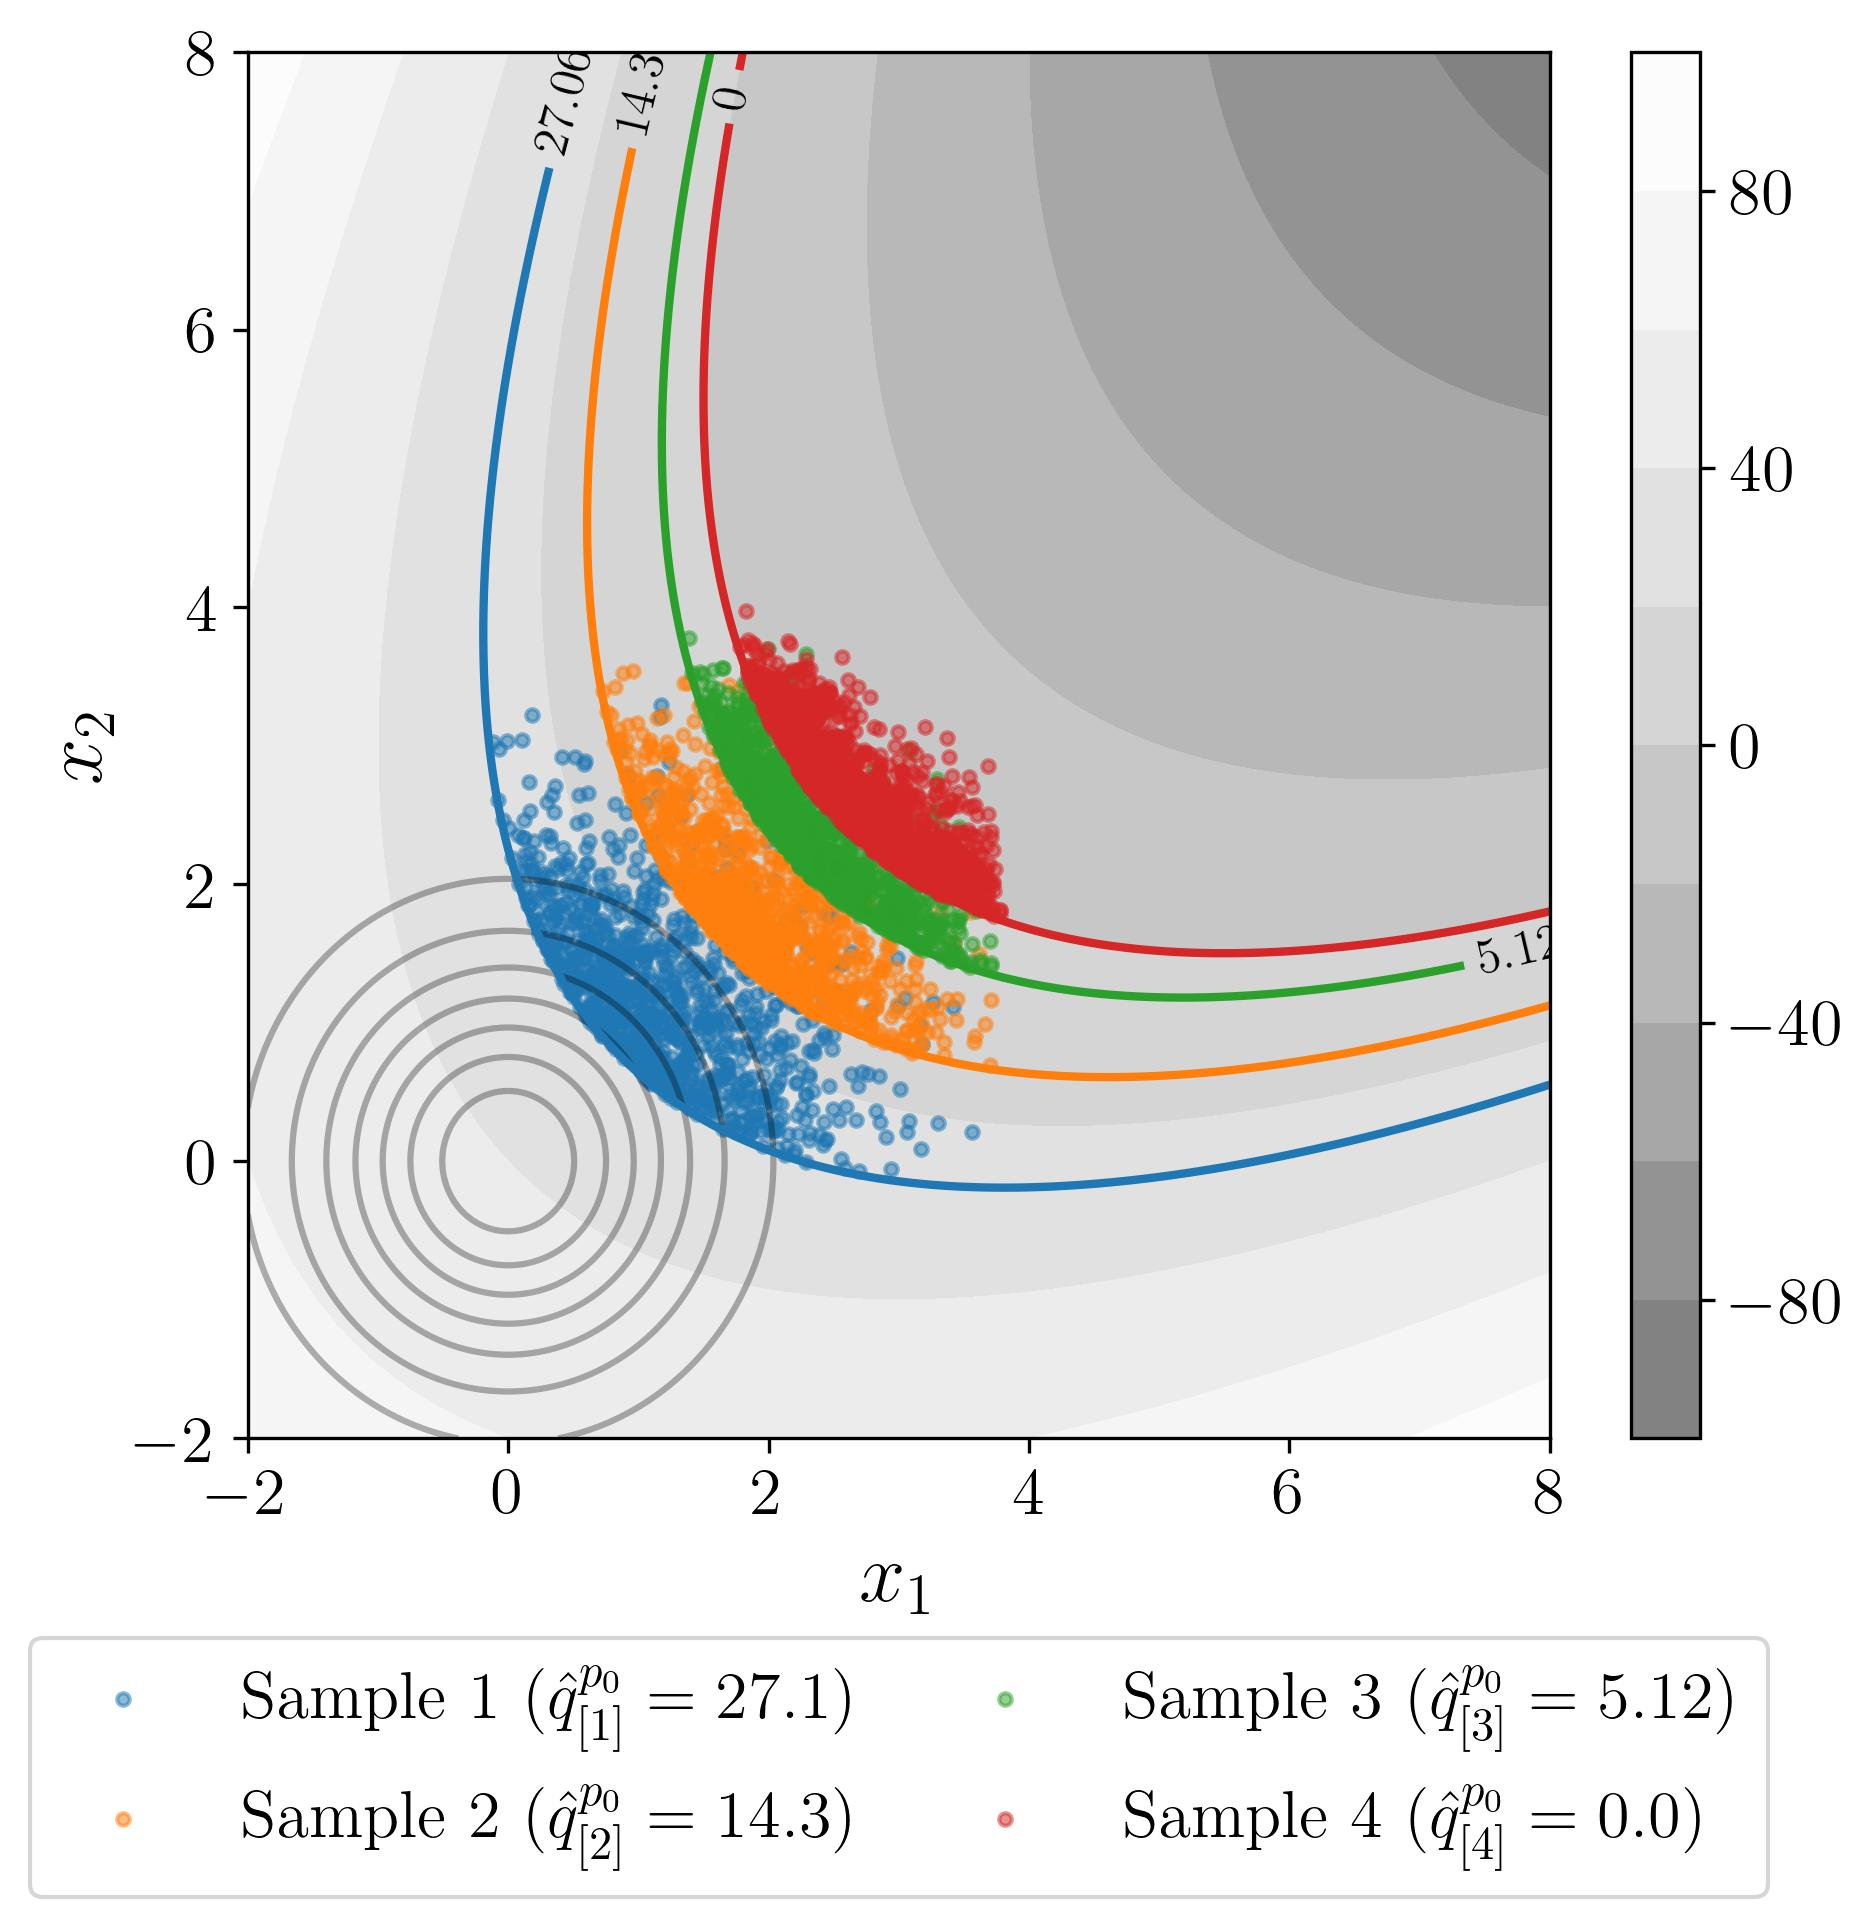
\includegraphics[width=\linewidth]{part3/figures/BANCS/bancs_parabolic.jpg}
        \caption{Test case \#1.}
    \end{subfigure}
    \begin{subfigure}[b]{0.49\linewidth}
        \centering
        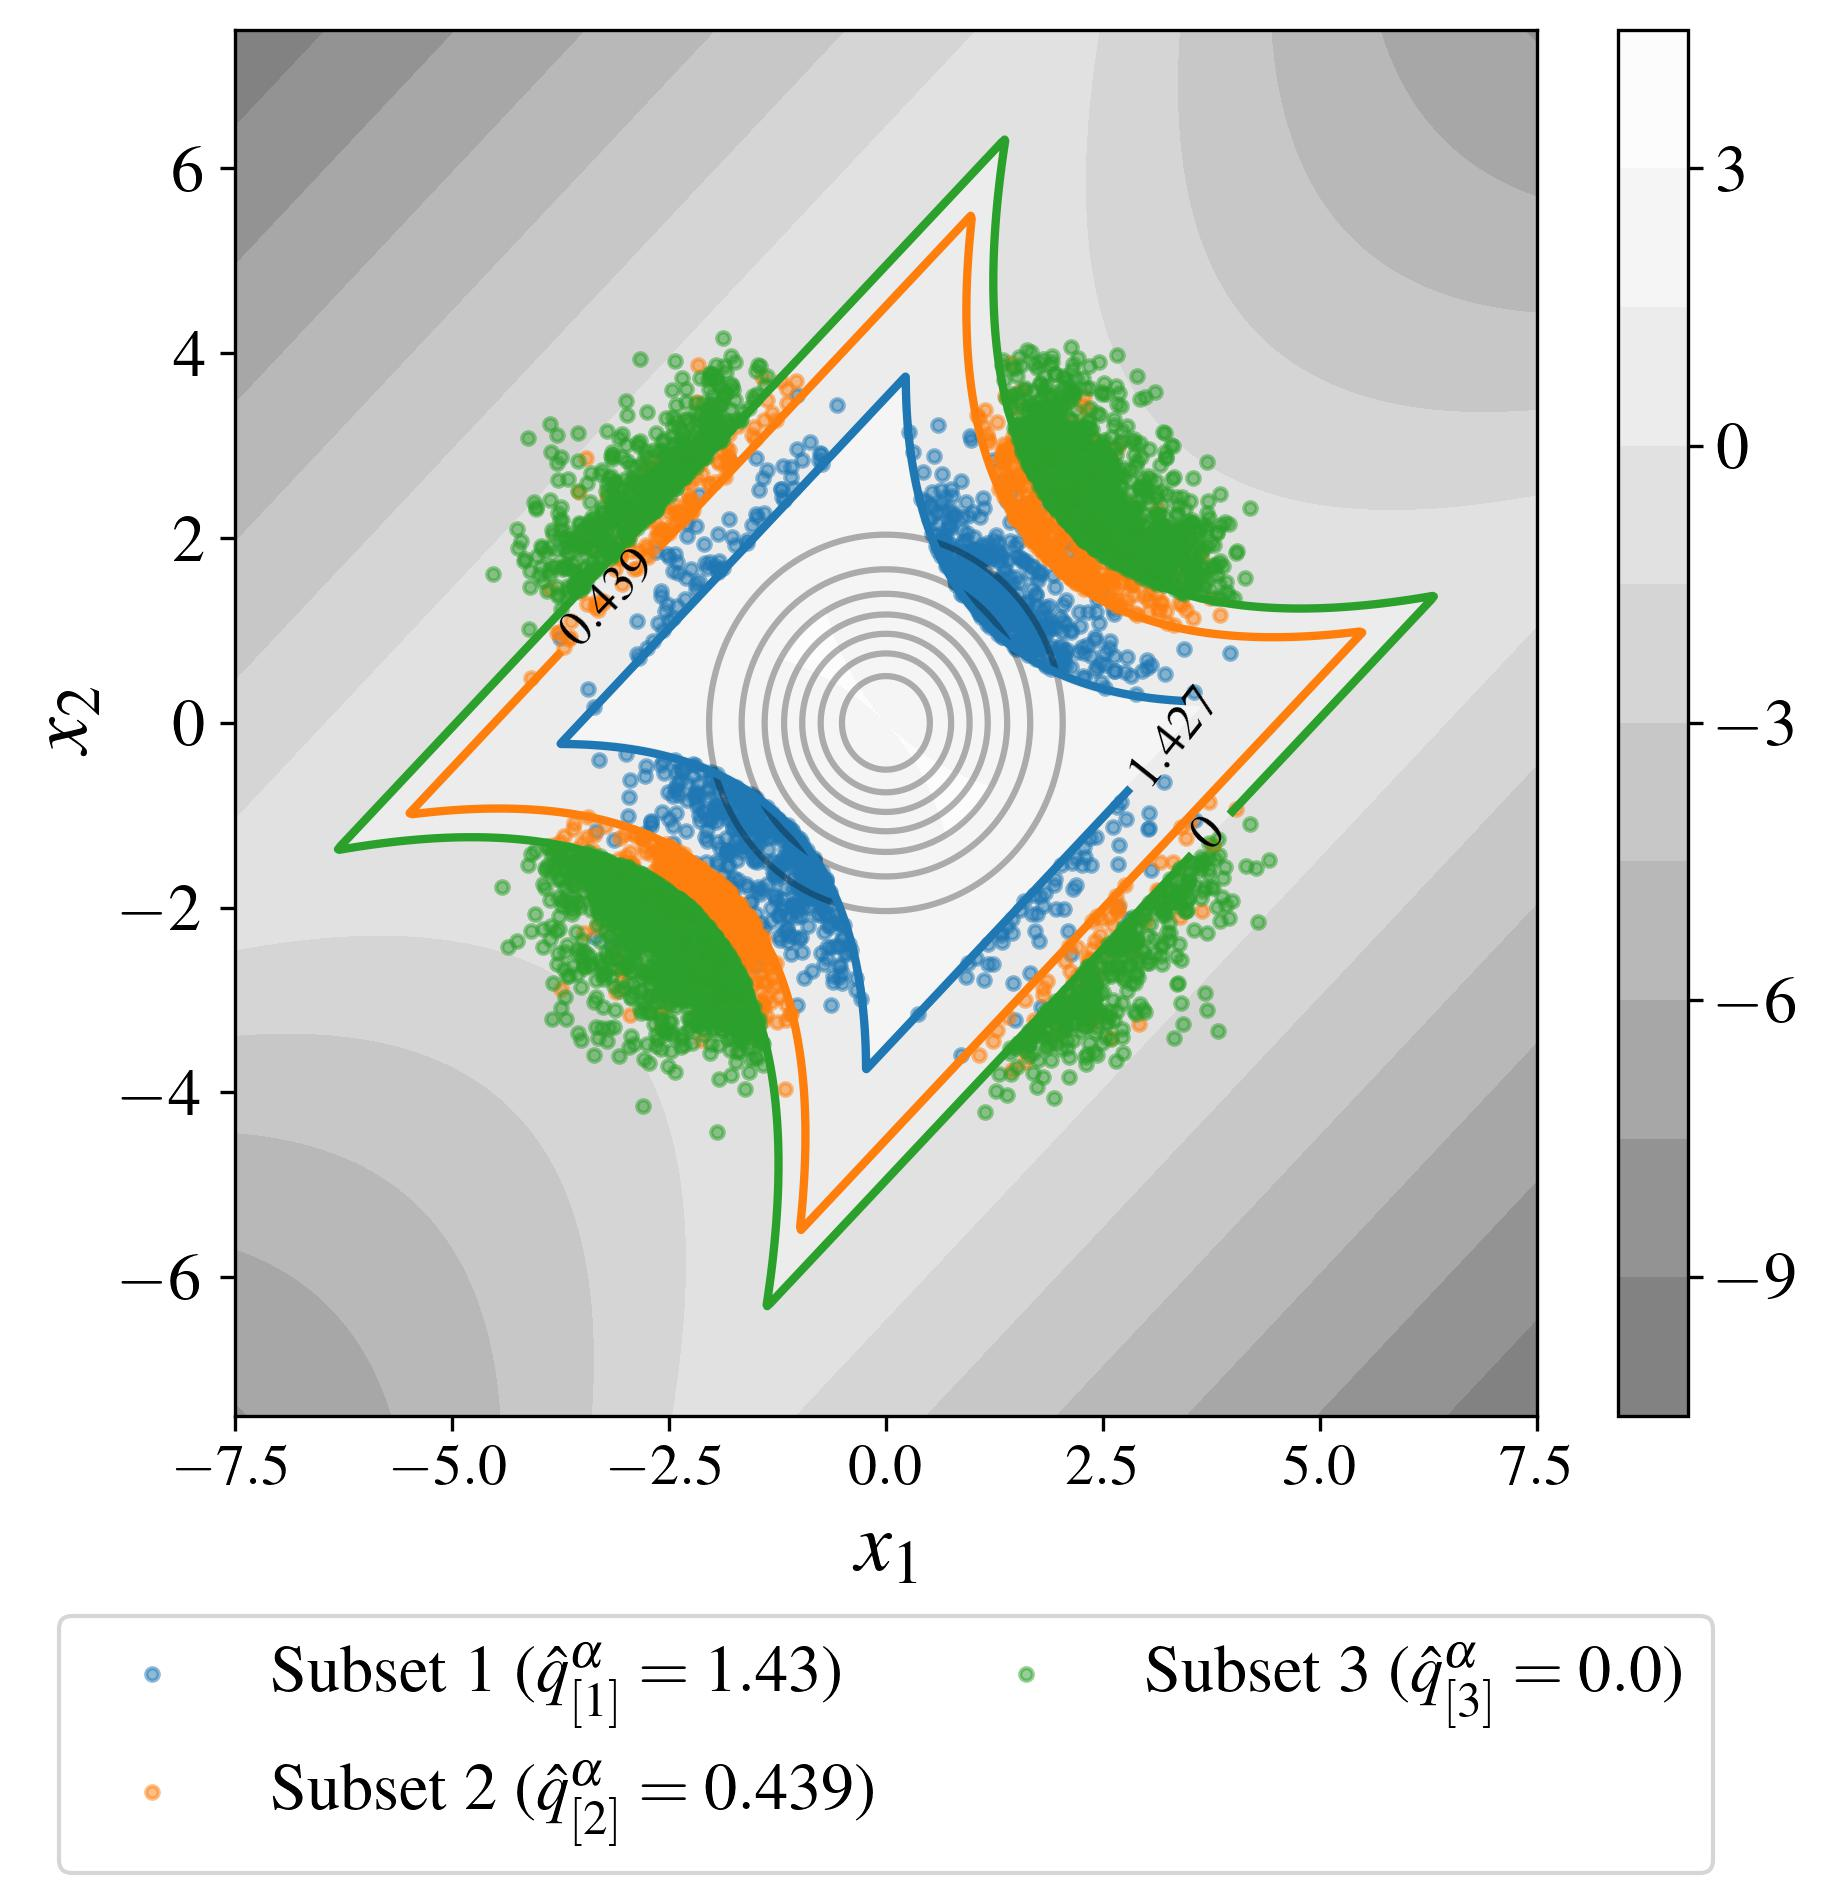
\includegraphics[width=\linewidth]{part3/figures/BANCS/bancs_4branch.jpg}
        \caption{Test case \#2.}
    \end{subfigure}
    \caption{Illustration of BANCS iterations for the two-dimensional reliability problems in test cases \#1 and \#2  (taking $N=10^4$ and $p_0=0.1$). 
    Only the samples exceeding the intermediary thresholds are represented.}
    \label{fig:2D_toycase_reliability}
\end{figure}


\begin{figure}
    \centering
    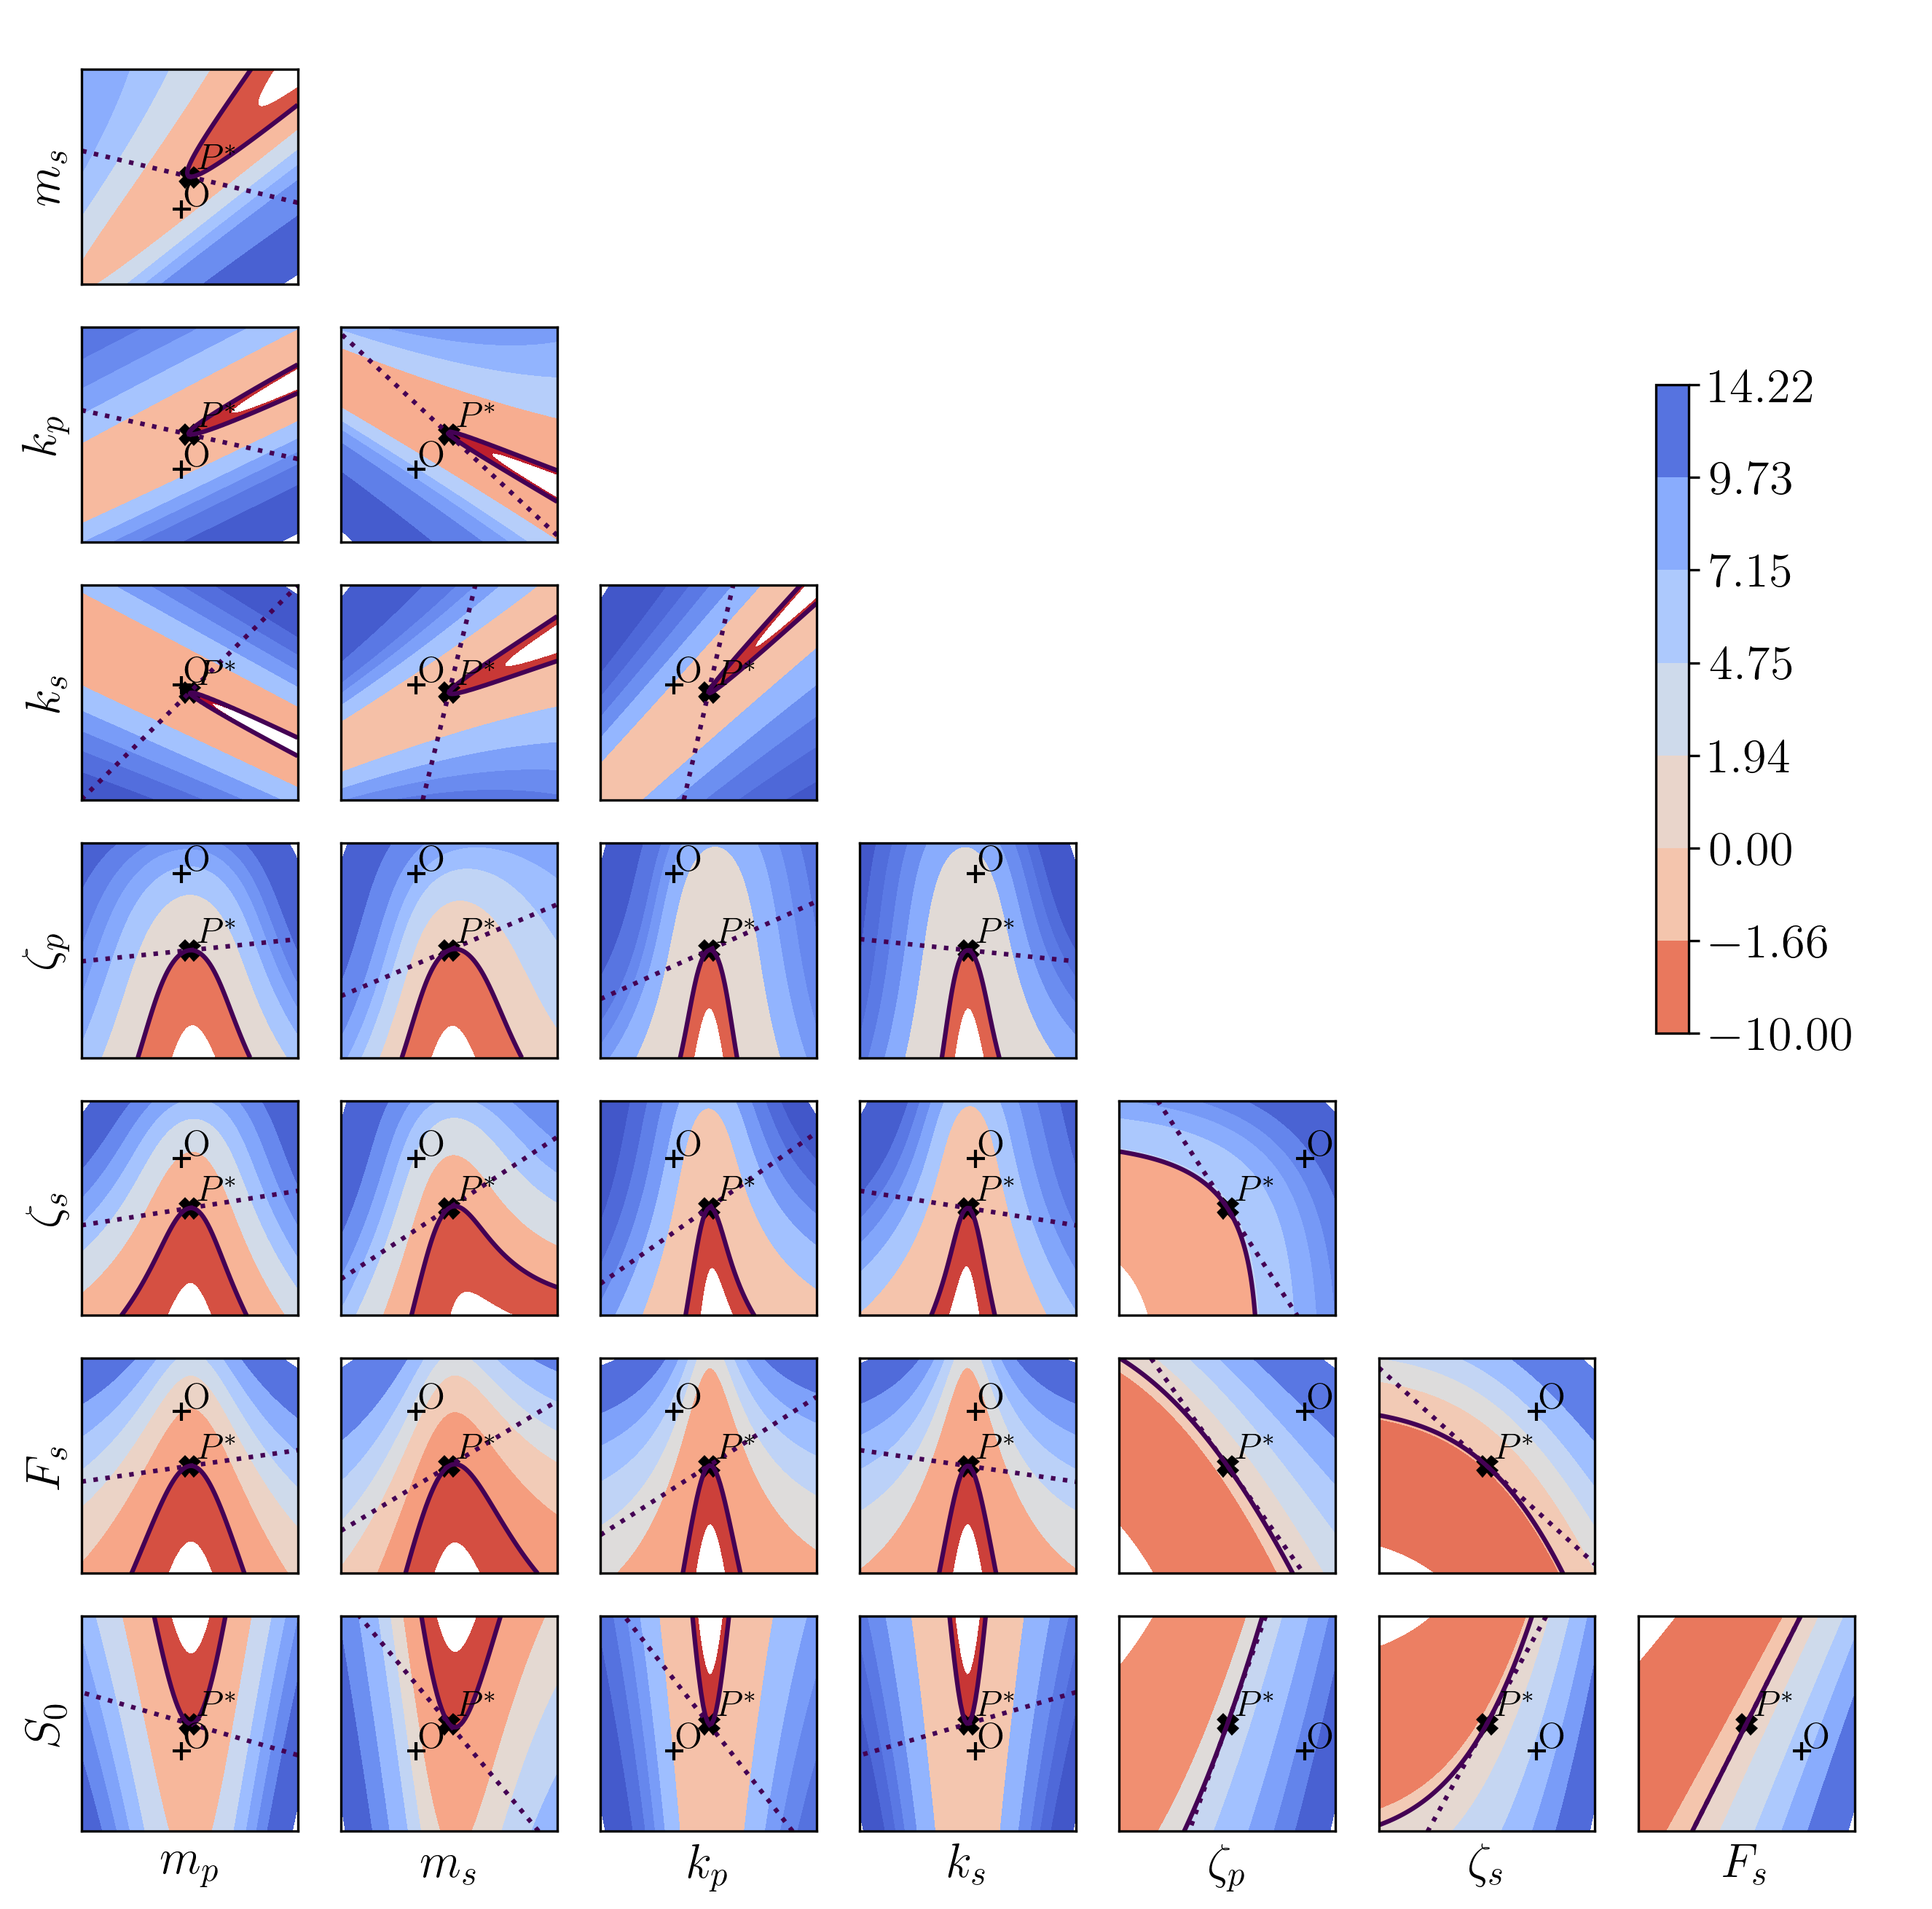
\includegraphics[width=0.7\textwidth]{part3/figures/BANCS/crosscut_oscillator.png}
    \caption{Cross-cut visualization of the limit-state function in test case \#5. 
    FORM's most-probable failure point $P^*$ is given by the black cross. 
    The LSF (full line) delimits the safe domain (in blue) and the failure domain (in red). 
    FORM approximation around $P^*$ (represented by the dashed lines).}
    \label{fig:crosscut_oscillator}
\end{figure}


\begin{figure}
    \centering
    \begin{subfigure}[b]{0.49\linewidth}
        \centering
        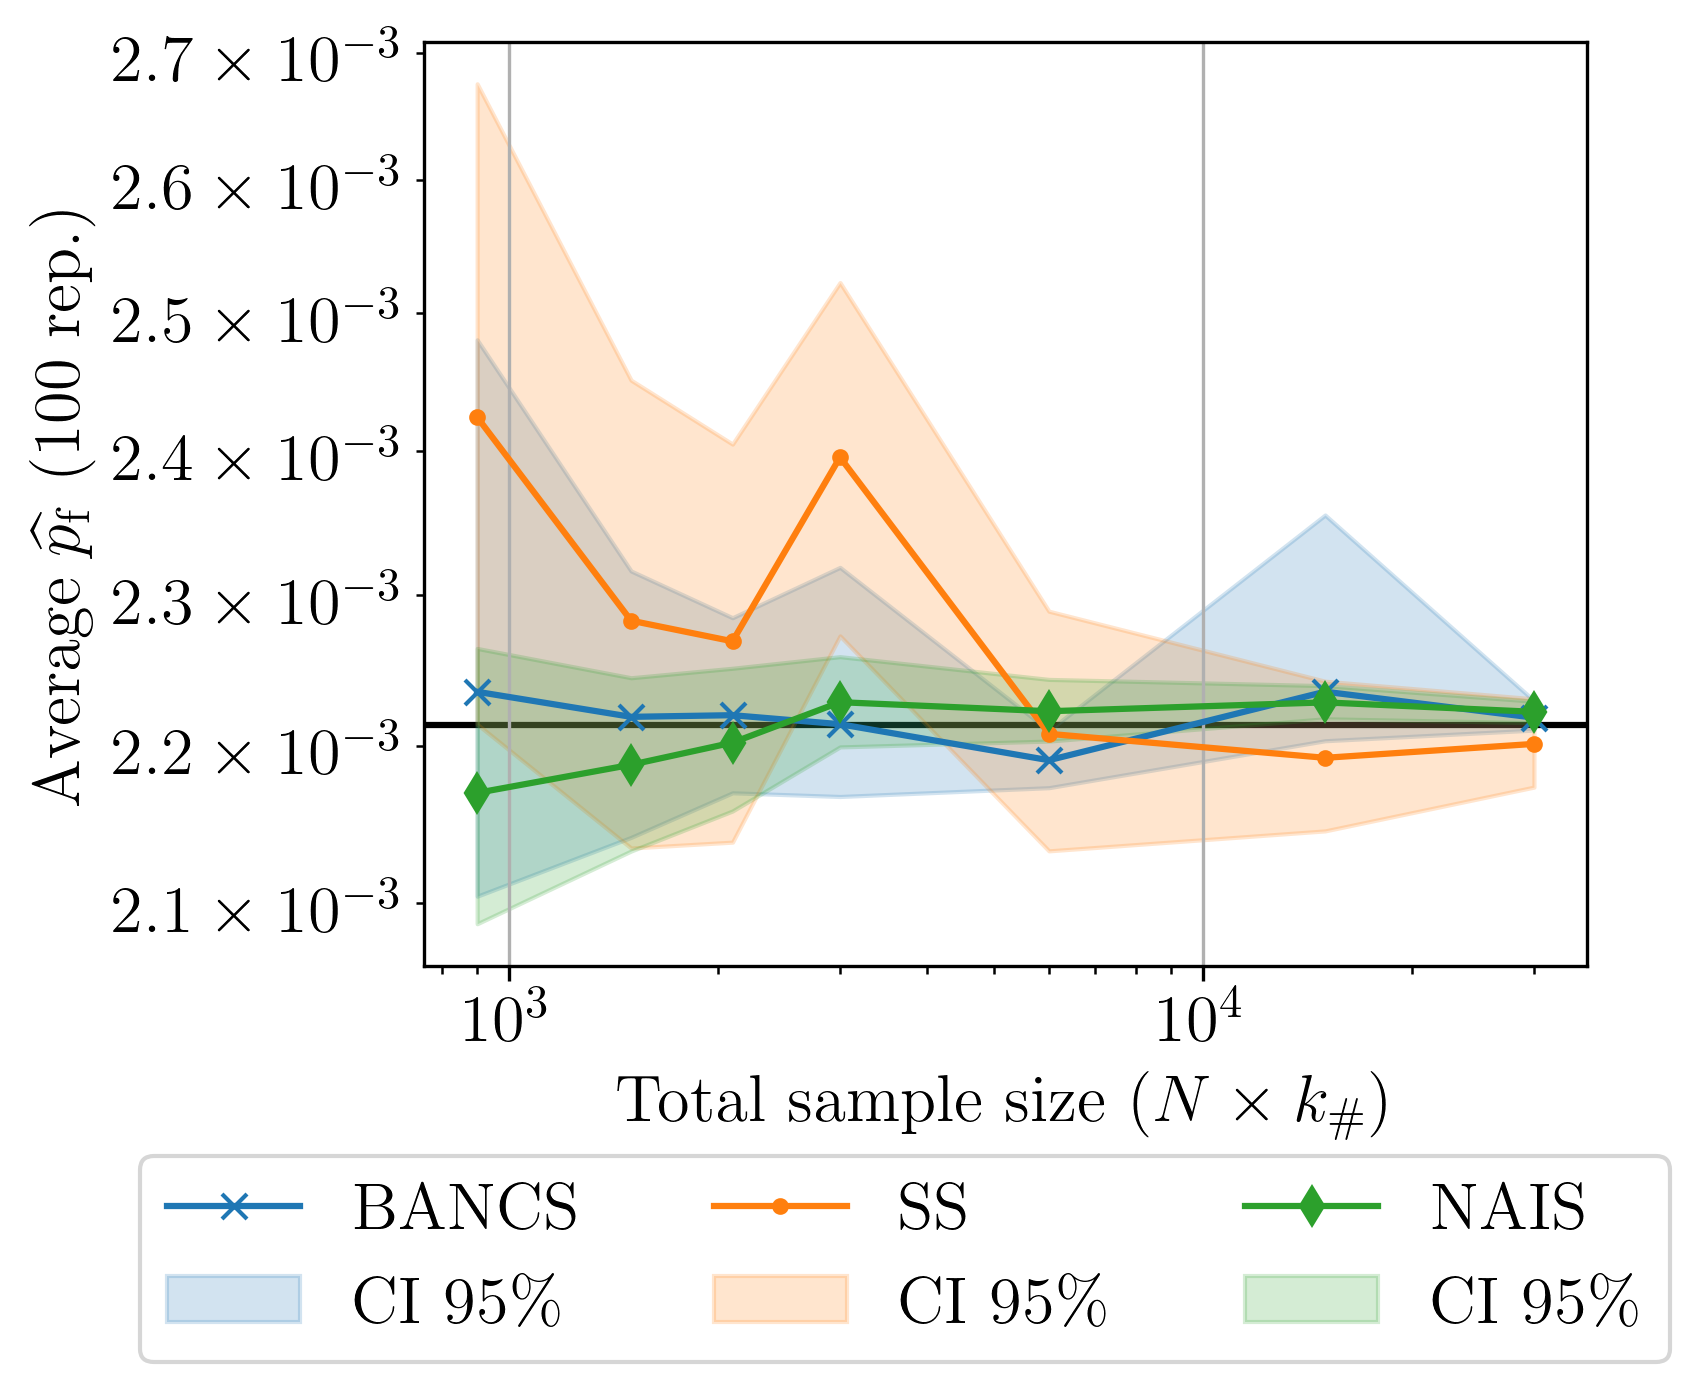
\includegraphics[width=\linewidth]{part3/figures/BANCS/RP4B_mean.png}
        \caption{Failure probability (test case \#2).}
    \end{subfigure}
    \begin{subfigure}[b]{0.47\linewidth}
        \centering
        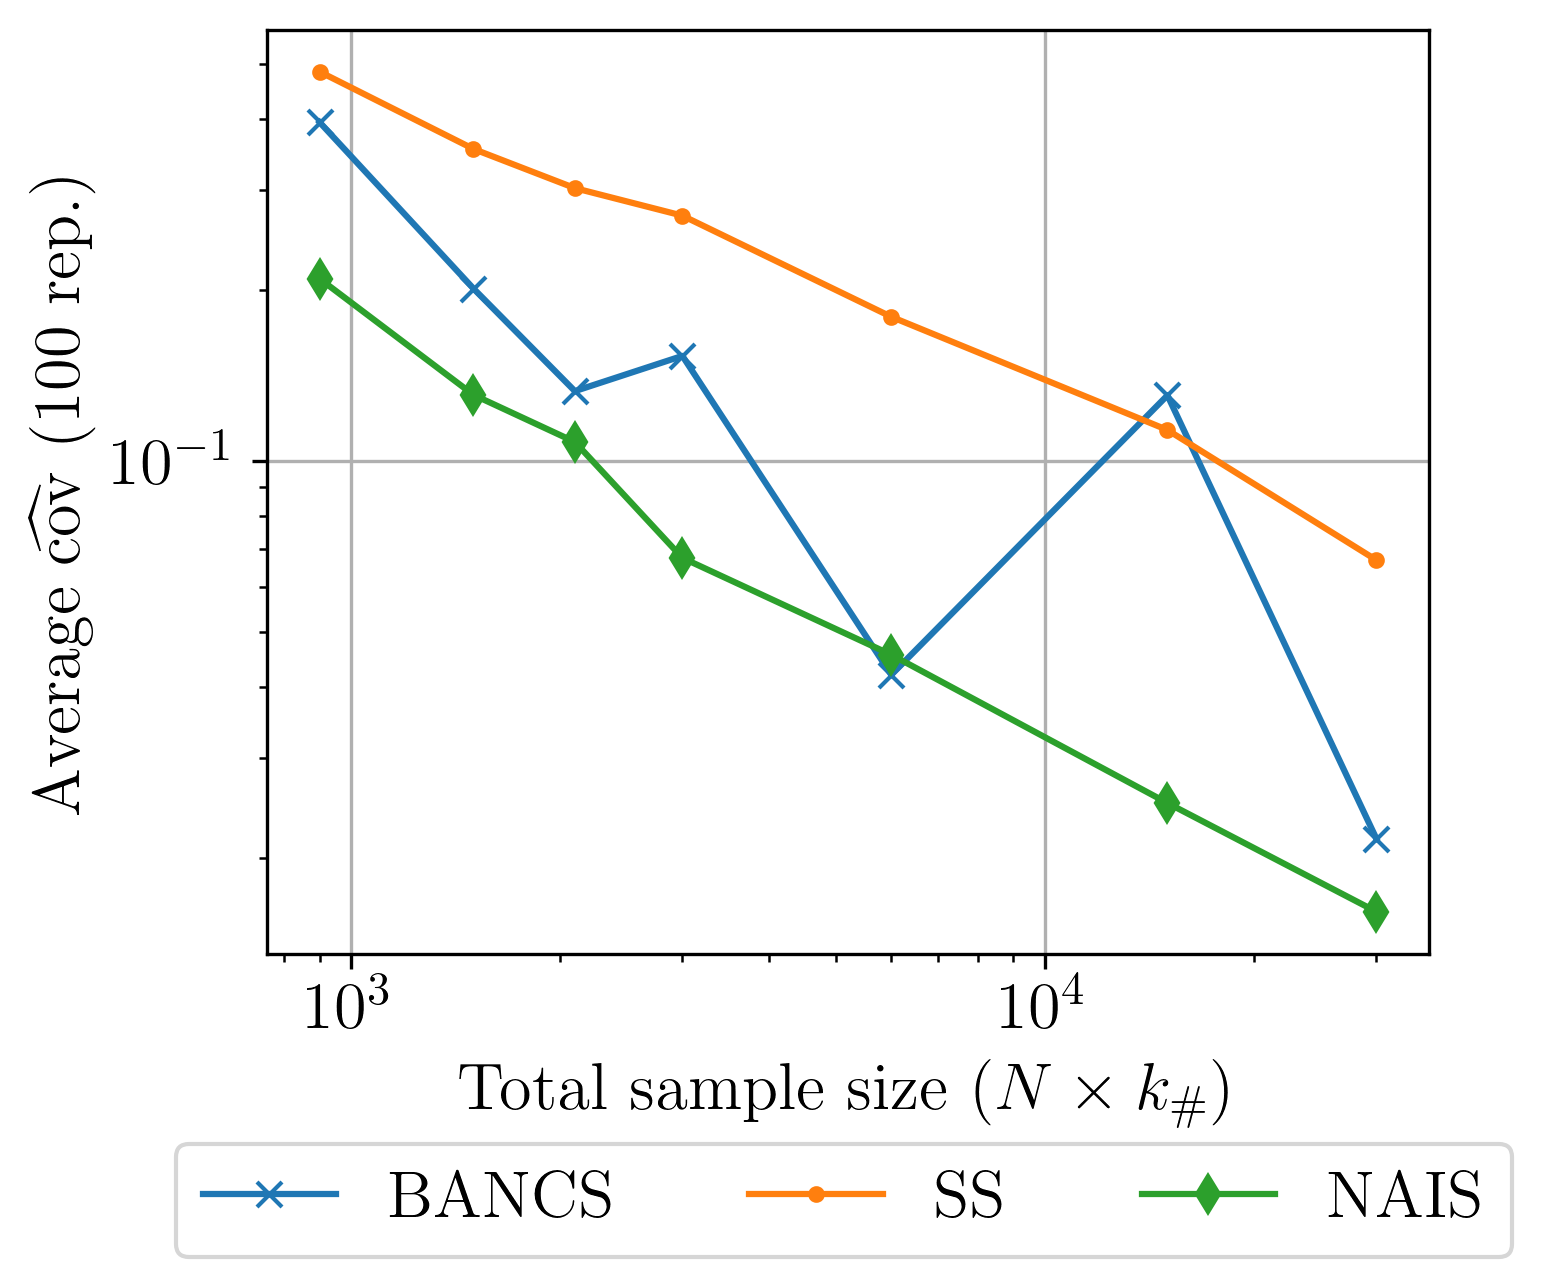
\includegraphics[width=\linewidth]{part3/figures/BANCS/RP4B_cov.png}
        \caption{Coefficient of variation (test case \#2).}
    \end{subfigure}
    \begin{subfigure}[b]{0.49\linewidth}
        \centering
        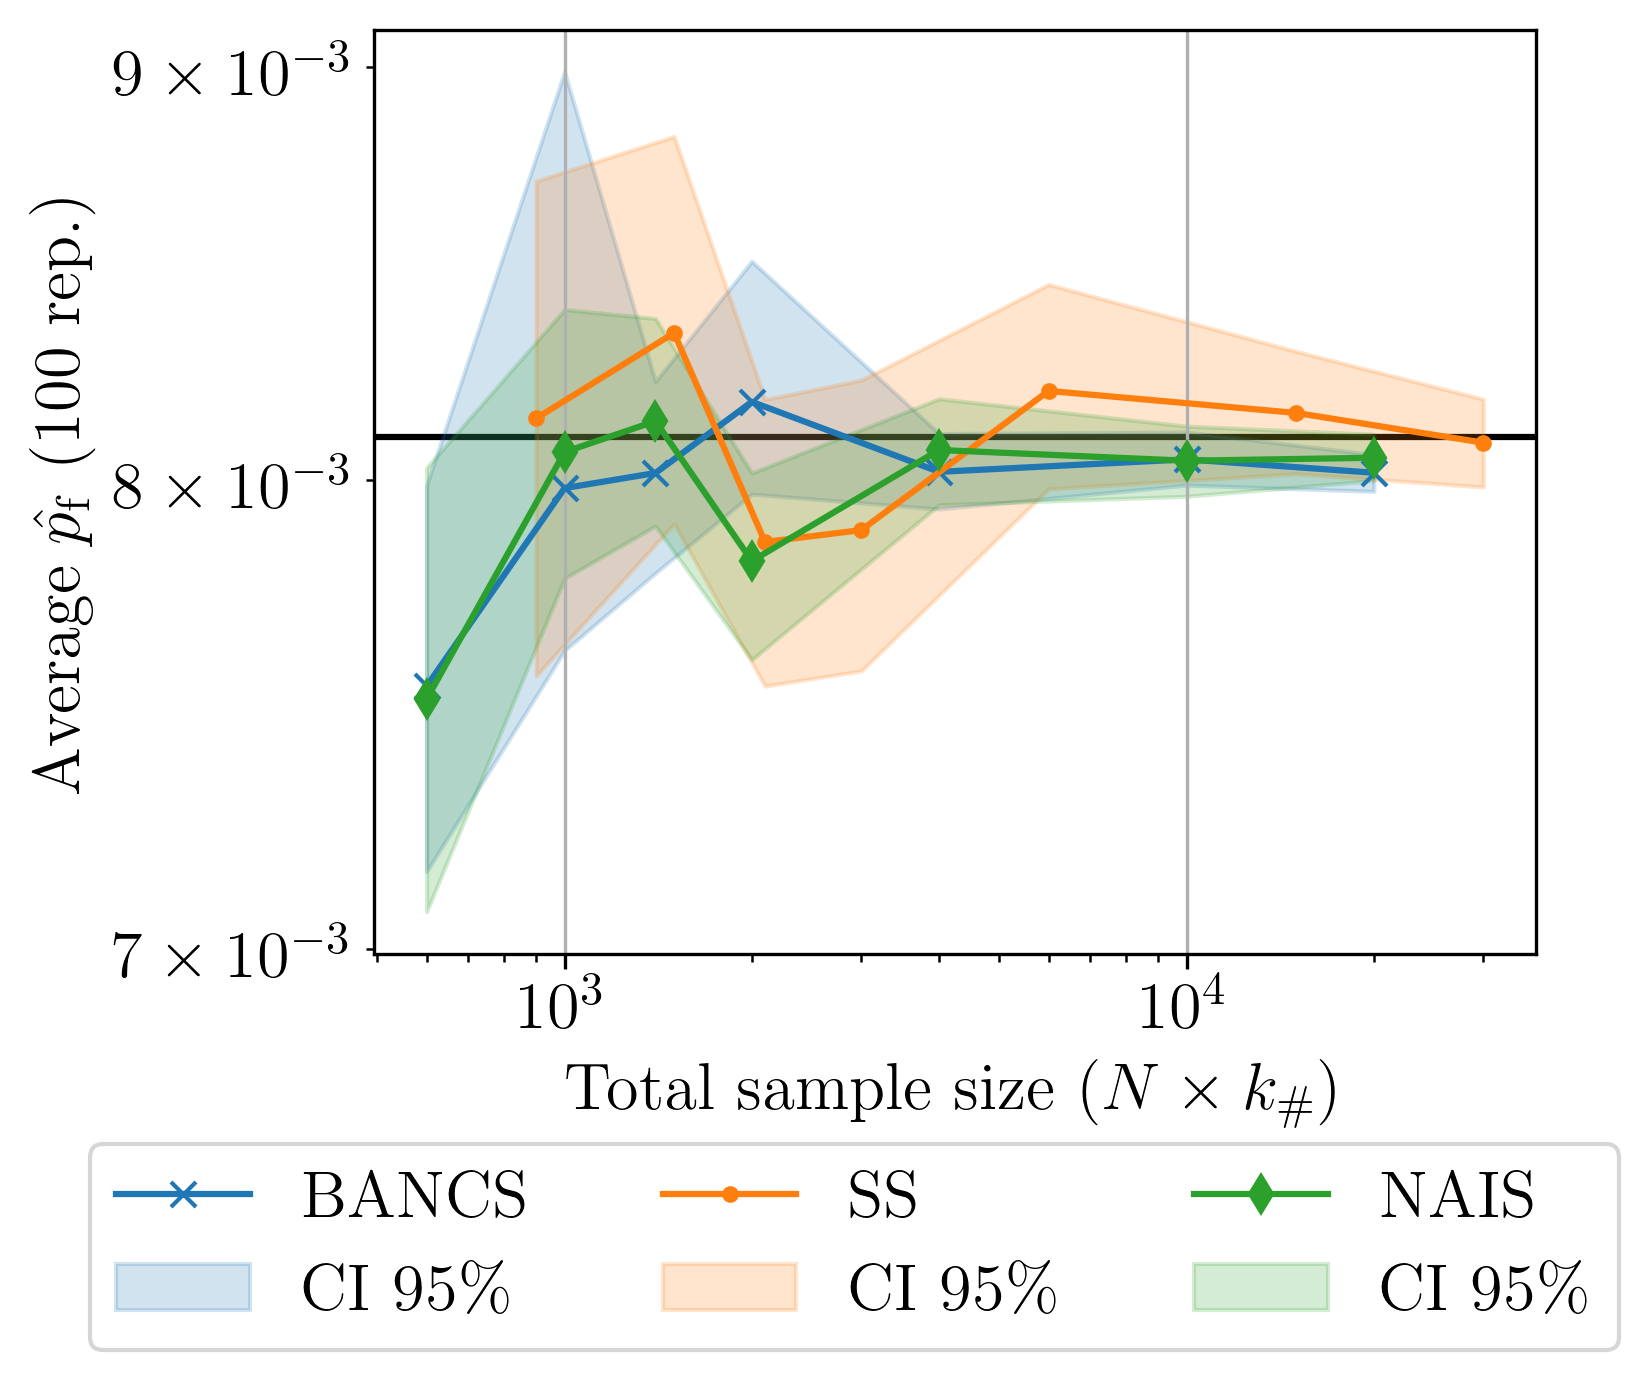
\includegraphics[width=\linewidth]{part3/figures/BANCS/RP38_mean.png}
        \caption{Failure probability (test case \#4).}
    \end{subfigure}
    \begin{subfigure}[b]{0.47\linewidth}
        \centering
        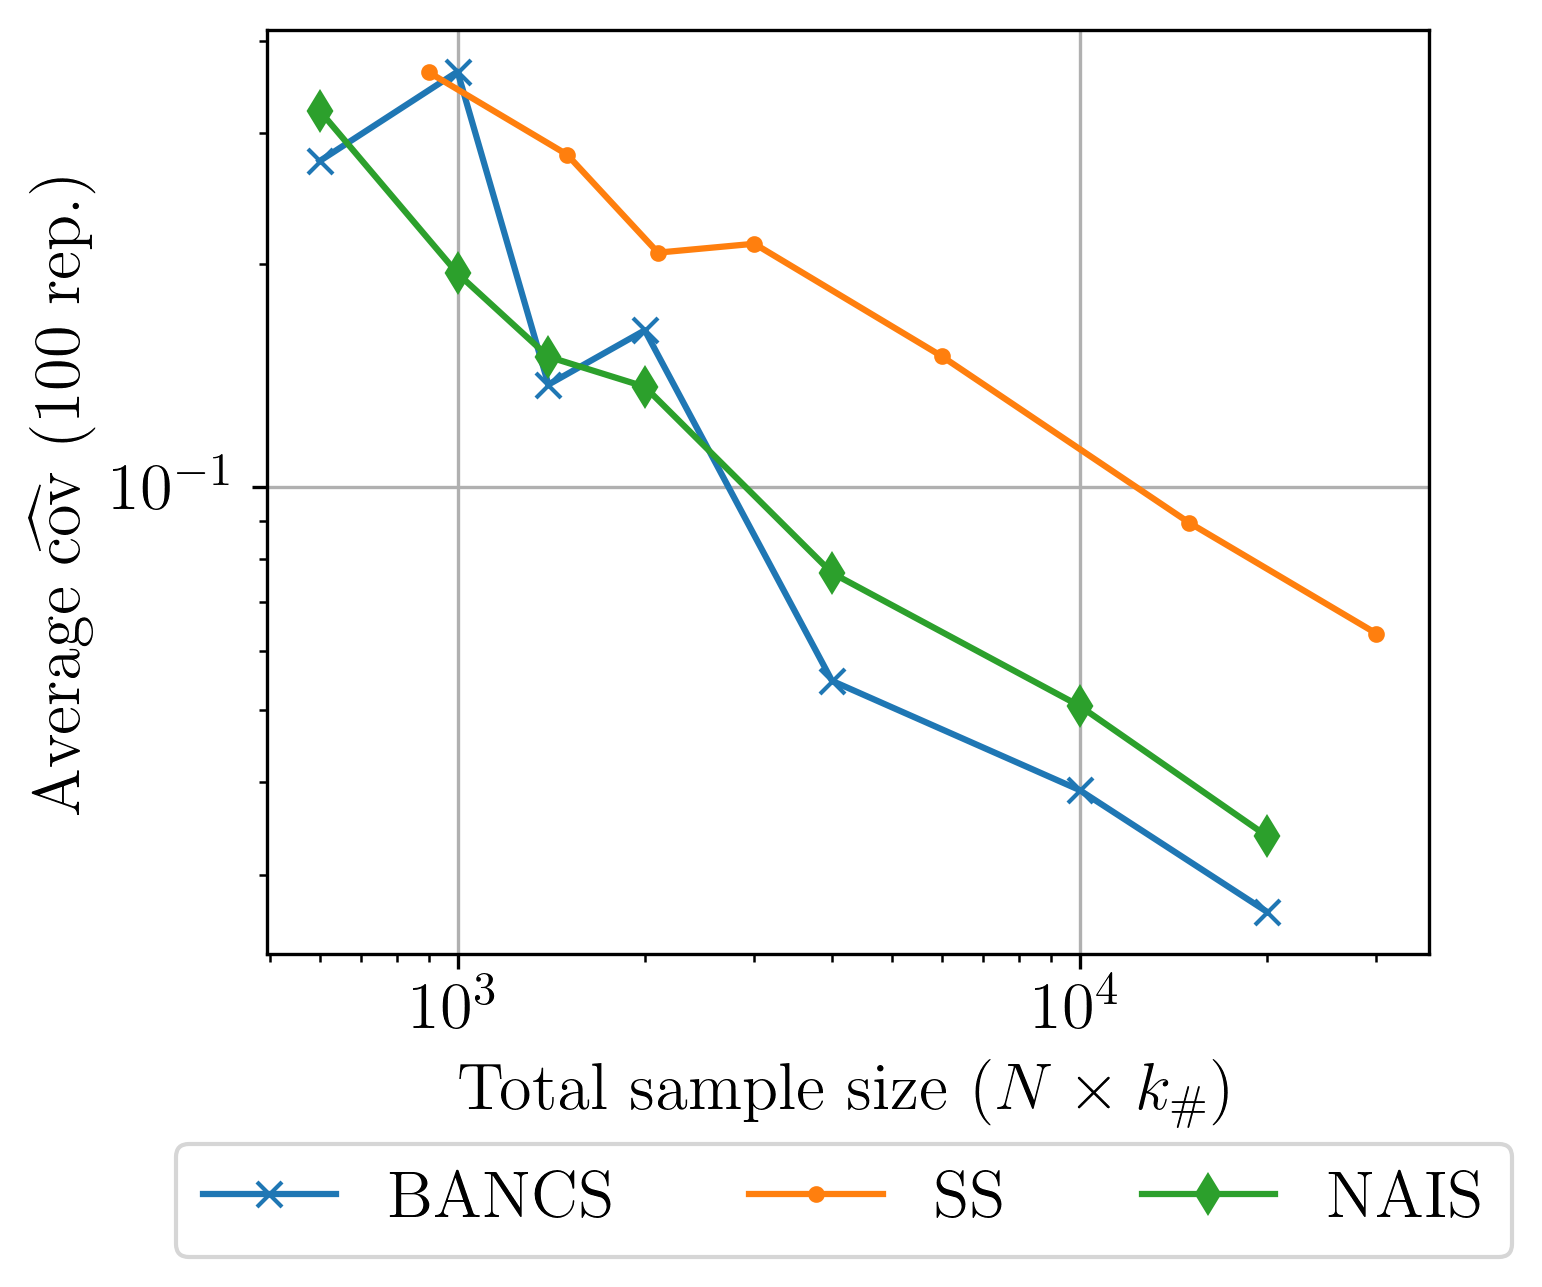
\includegraphics[width=\linewidth]{part3/figures/BANCS/RP38_cov.png}
        \caption{Coefficient of variation (test case \#4).}
    \end{subfigure}

    \begin{subfigure}[b]{0.49\linewidth}
        \centering
        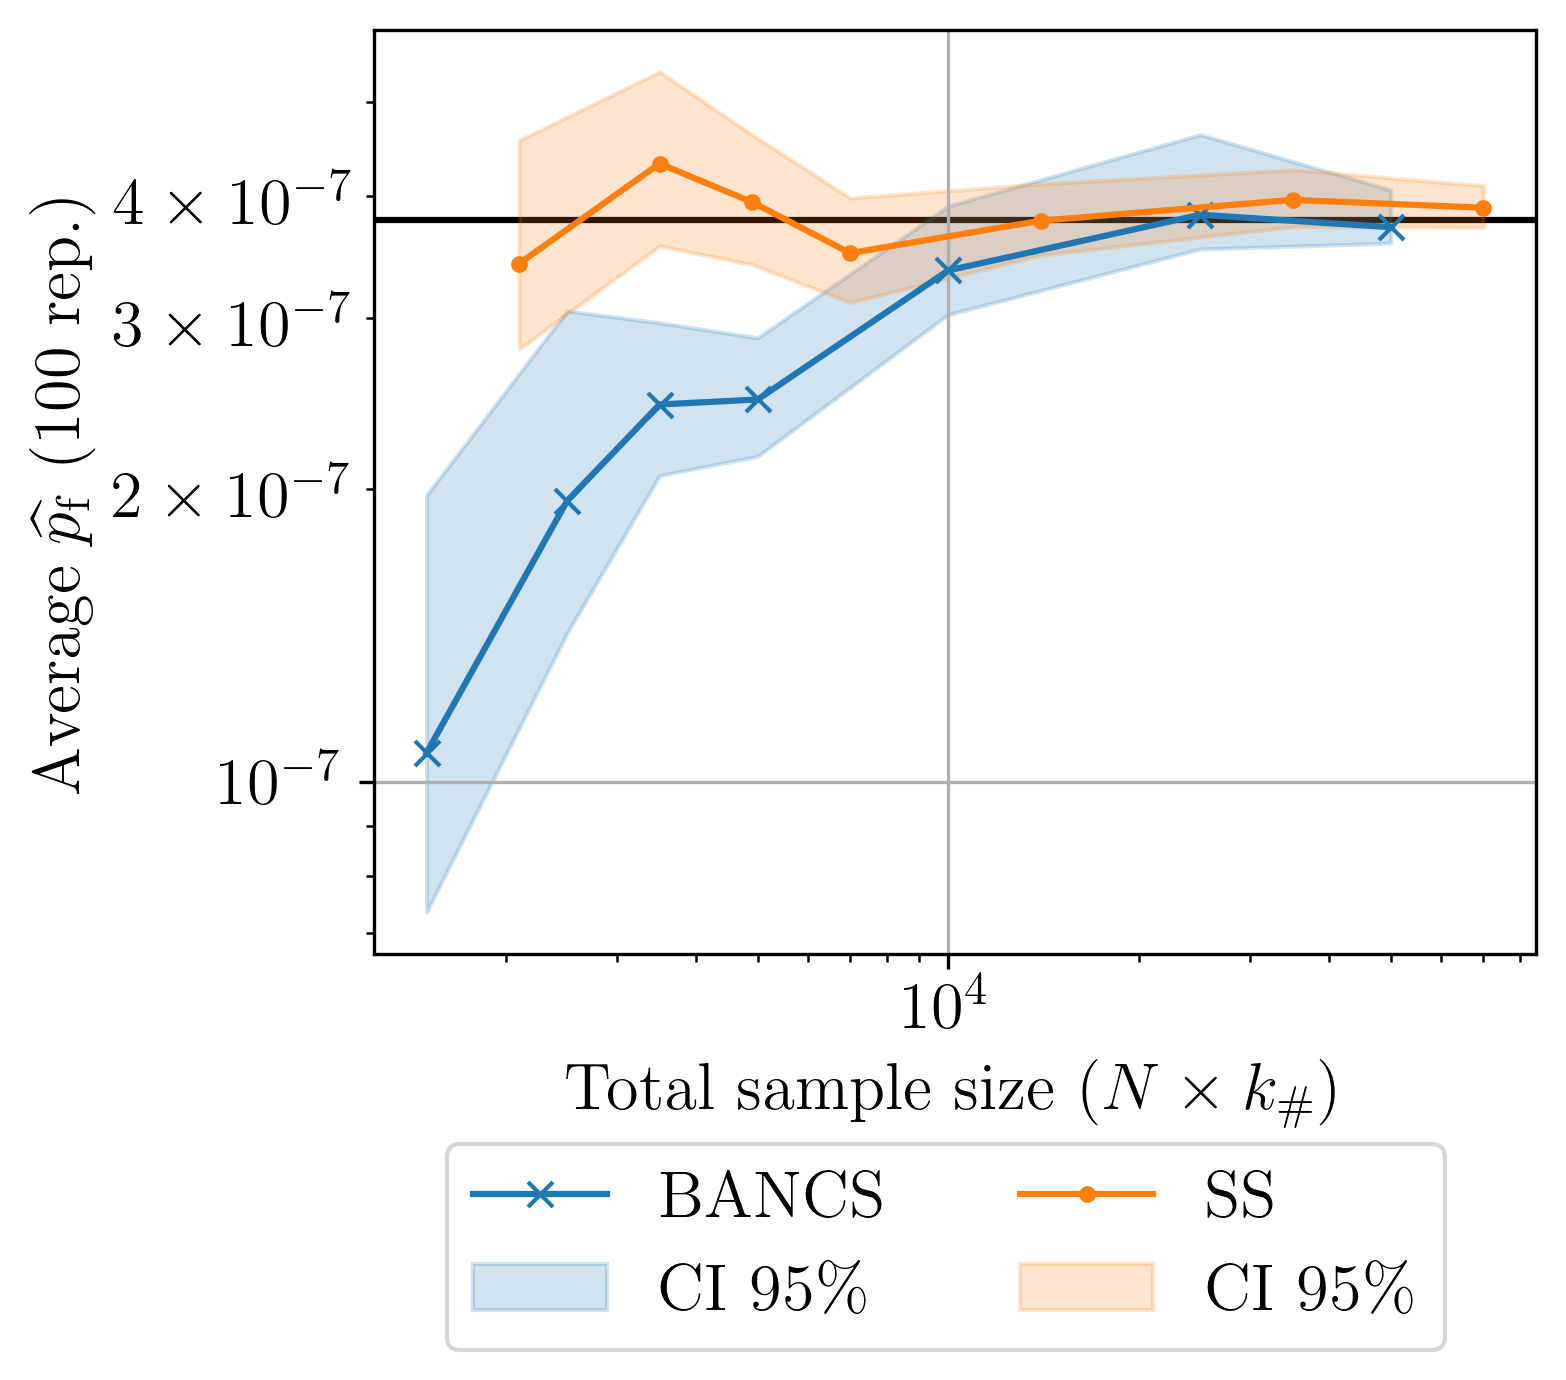
\includegraphics[width=\linewidth]{part3/figures/BANCS/Oscillator_mean.png}
        \caption{Failure probability (test case \#5).}
    \end{subfigure}
    \begin{subfigure}[b]{0.47\linewidth}
        \centering
        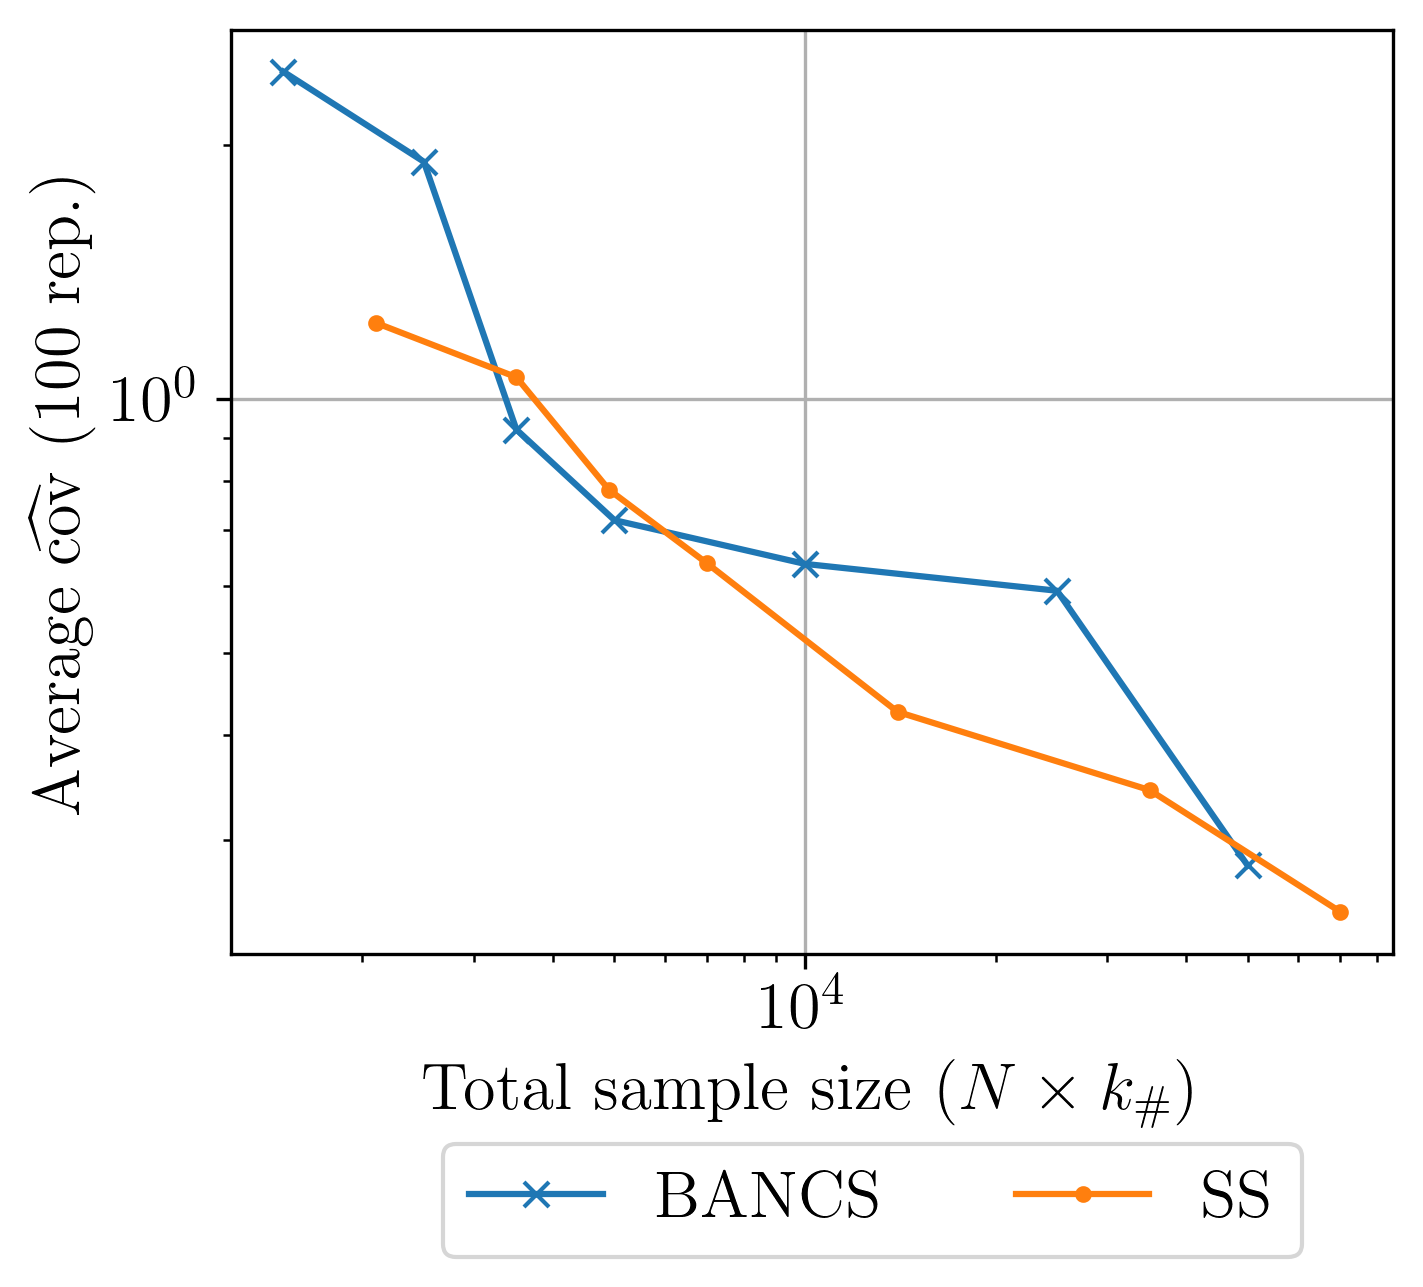
\includegraphics[width=\linewidth]{part3/figures/BANCS/Oscillator_cov.png}
        \caption{Coefficient of variation (test case \#5).}
    \end{subfigure}
    \caption{Reliability analysis benchmark between BANCS, SS and NAIS using 100 repetitions of each experiment (with $p_0=0.1$ for every methods). 
                The confidence intervals are obtained by bootstrap on the repetitions. 
                The reference failure probabilities are represented by the horizontal black lines.}
    \label{fig:bancs_benchmark}
\end{figure}

%============================================================%
%============================================================%
\section{Reliability-oriented sensitivity analysis}\label{sec:bancs_rosa}
%============================================================%
%============================================================%


As introduced in Section~\ref{sec:gsa}, GSA can be viewed as a tool to assess the global impact of the input variability on the output variable of interest. 
When estimating quantities of interest related to the output distribution's tail (typically, risk measures such as quantiles or failure probabilities), the analysis should be dedicated to the subdomain of interest (e.g., the failure domain). 
In other words, the global influence of the inputs (e.g., on the output's variance) may be different from their reliability-oriented influence (e.g., their influence on a rare event probability). 

To address this issue, the topic of \textit{reliability-oriented sensitivity analysis} (ROSA) is an active research field where several GSA methods were adapted to the analysis of risk measures. 
Historically, the FORM importance factors represent a first importance measure adapted to ROSA. 
However, it is only a local measure (obtained as a post-processing of FORM), since it captures the influence near the most-probable failure point.  
Later on, global sensitivities such as the Sobol' indices were adapted to the indicator function \citep{wei_2012_rosa,chabridon_2018_thesis,perrin_2019_rosa}. 
Recently, \citet{papaioannou_2021_rosa_form} discussed the link between the importance factors and the Sobol' indices on the indicator. 
Moment-independent importance measures were also applied to study the sensitivity of reliability. 
For example, \citet{daveiga_2015} suggested the use of Hilbert-Schmidt indepencence criterion (HSIC) for reliability. 
This idea was further explored by \citet{marrel_chabridon_2021} who distinguished two categories of ROSA with different purposes: 
\begin{itemize}
    \item \textit{Target sensitivity analysis} (\abv{tsa}), measuring the influence of input variables w.r.t. exceeding a threshold on the output; 
    \item \textit{Conditional sensitivity analysis} (\abv{csa}), studying the impact of input variables within the restricted domain (i.e., conditionally to this domain).
\end{itemize}
Finally, several new indices have been proposed in the ROSA context to deal with dependent inputs, such as the ``target Shapley effects'' by \citet{ilidrissi_2021_rosa}, whose estimation has been further improved by \citet{demange_2023_ijuq}. More recently, \citet{ehre_2024_vb_rosa} proposed a new set of Sobol' indices on the indicator function suited to this context via extending the previous work of \citet{mara_tarantola_2012}.

All in all, this section aims at illustrating the estimation of HSIC-based TSA and CSA indices as a simple post-processing of BANCS. 
After estimating a rare event probability with BANCS, a set of i.i.d. samples (each with size $N$) is available. 
These consecutive samples gradually move towards the failure domain and become rarer from the perspective of the initial input distribution. 
This section first recalls the TSA and CSA adaptation from \citet{marrel_2018} and \citet{marrel_chabridon_2021} of the HSIC indices, whose formulation was introduced for GSA in Section~\ref{sec:gsa}.
Then, the computation of the so-called ``target-HSIC'' and ``conditional-HSIC'' indices is presented as a simple post-precessing of the BANCS reliability analysis. 
This procedure is illustrated on test cases \#3 and \#5. 


%============================================================%
\subsection{Target and conditional HSIC indices}
%============================================================%

A first approach for TSA is to directly apply any sensitivity measure to the binary variable $\1_{\{g(\bX) \leq \yth\}}$. 
However, this strategy does not distinguish points in the vicinity of the LSF from points that are far from this border. 
In the present work, a threshold relaxation using the weight transformation proposed in \citet{marrel_2018} and further discussed in \citet{marrel_chabridon_2021} is applied to gather more information. 
Let us consider the weight function $w_{\iF}: \R \rightarrow [0, 1]$ such that $w_{\iF}(y) = \exp(-d_{\iF}(y)/s)$, where $d_{\iF} = \mathrm{inf}_{y'\in \iF} \Vert y -y' \Vert$ is a distance to the border and $s\in\R$ is a smoothing parameter. 

Then, a TSA measure can be defined as the result of any sensitivity measure applied between the random inputs $\bX$ and $w_{\iF}(Y)$. 
In our case, the target-HSIC (T-HSIC) and its respective normalized version, called the target $R^2_{\HSIC}$ ($T \mhyphen R^2_{\HSIC}$) are defined as: 
\begin{subequations}
    \begin{align}
        T \mhyphen \HSIC(X_j, Y) & = \HSIC(X_j, w_{\iF}(Y)) = \MMD^2(\P_{(X_j, w_{\iF}(Y))}, \P_{X_j} \otimes \P_{w_{\iF}(Y)})\, ,\\
        T \mhyphen R^2_{\HSIC}(X_j, Y) &= \frac{T \mhyphen \HSIC(X_j, w_{\iF}(Y))}{\sqrt{T \mhyphen \HSIC(X_j, X_j) \, T \mhyphen \HSIC(w_{\iF}(Y), w_{\iF}(Y))}}\, .
    \end{align}
\end{subequations}
The stronger the dependence, the more $X_j$ is influential on the occurrence of the rare event $\{Y\in\iF\}$.  
Another advantage of applying the threshold relaxation is that any real-value kernel can be used to define the HSIC. 

As for the conditional indices, let us define the probability of $Y$ conditionally to the rare event $\{Y \in \iF\}$, considering the measurable space $(\Omega, \iA)$:
\begin{equation}
    \P_{Y|\{Y\in\iF\}}(A) = \frac{\int_{A} \1_{g(\bX)\leq0}(y) \, \dd \P_Y}{\pf}\,, \quad \forall A \in \iA\,.
\end{equation}
After applying the same threshold relaxation as earlier, one can write $\forall A \in \iA$: 
\begin{equation}
    \P_Y^{w_{\iF}}(A)= \frac{\int_A w_{\iF}(y) \, \dd \P_Y}{\int_{\Omega} w_{\iF}(y) \, \dd \P_Y} \, ,
\end{equation}
and the conditional expectation: 
\begin{equation}
    \E[Y|Y \in \iF] = \E_{Y\sim\P_Y^{w_{\iF}}}[Y] = \frac{\int_\Omega y w_{\iF}(y) \, \dd \P_Y}{\int_{\Omega} w_{\iF}(y) \, \dd \P_Y}\, .
\end{equation}
Using this expression, the following conditional HSIC is proposed by \citet{marrel_2018} and further explored in \citet{marrel_chabridon_2021}:
\begin{subequations}
    \begin{align}
        C \mhyphen \HSIC(X_j, Y) & = \HSIC_{(X_j, Y) \,\sim\, \P_{(X_j, Y)}^{w_{\iF}}} (X_j, Y) \, ,\\
        C \mhyphen R^2_{\HSIC}(X_j, Y) &= \frac{C \mhyphen \HSIC(X_j, Y)}{\sqrt{C \mhyphen \HSIC(X_j, X_j) \, C \mhyphen \HSIC(Y, Y)}}\, .
    \end{align}
\end{subequations}
Note that the conditional indices defined hereabove may rely on both a filtering of the output (as in TSA) through the use of the $w_{\iF}$ function, which thus induces a weighting of the samples in the estimator (see \citet{marrel_chabridon_2021} for more details about these estimators).

As a remark, one can notice that the $R^2_{\HSIC}$ indices (either in their global, target or conditional versions) are normalized indices (i.e., lying in $[0,1]$) which can be useful for a pragmatic ranking of the most influential variables. However, from a theoretical perspective, the observed values of these indices (and thus, sometimes, the rankins) may vary with respect to the kernel choice (i.e., the family and the estimated parameters) which can be disturbing for the analyst.

In addition, from the estimation point of view, HSIC measures are computed, in practice, from a finite set of realizations. Therefore, the estimates might fluctuate, and the obtained values could be close to zero, but not properly equal to zero. As shown in \citet{delozzo_2016_hsic_test}, statistical hypothesis testing can be used in order to strengthen the decision process regarding the values of the indices (and thus make the screening more robust). Without going too much into details (see, e.g., \citet{chabridon_iooss_marrel_2020} for a brief presentation of these tests), depending on the nature of the analysis and the sample size, two kinds of tests are available. On the one hand, tn both TSA or CSA contexts, and even for samples that are of low or moderate sizes, the so-called ``permutation-based test'' proposed by \citet{delozzo_2016_hsic_test} is available. It consists in repeating several estimation of HSIC indices while permutating the output values. On the other hand, as soon as the sample size is large enough (this assumption needs to be considered carefully), the ``asymptotic regime'' lead to an asymptotic version of the test, which consists in approximating the law of test statistic as a gamma random variable. Thus, the test reduces to the evalutation of an analytic equation to compute the p-value. However, such a result is only valid for global and target analyses, not for the conditional one.
%Thus, as discussed in \citet{chabridon_bepu_2020}, the ranking should be assessed by combining both information from the indices and the p-values obtained from 
%Statistical tests are the only robust way of screening variables w.r.t. the quantity of interest. 
%In the context of TSA, the asymptotic tests proposed by \citet{gretton_2006} are well suited to the sample sizes encountered in reliability analysis. 
%However, the asymptotic approach no longer holds for CSA, which is replaced by the permutation-based statistical test proposed by \citet{delozzo_2016_hsic_test}.
%Note that the HSIC generally do not require independence of the samples but the permutation tests do. 

The respective estimators of all indices are provided in \citet{marrel_chabridon_2021} and their implementation is available in \ot.
Unlike Sobol' indices, the HSIC estimation is realized on the same sample for every variable $X_j$. 
This property allows us to apply HSIC TSA and CSA to the samples evaluated during the BANCS reliability analysis.


%============================================================%
\subsection{ROSA as a post-processing of a reliability analysis by BANCS}
%============================================================%

After assessing a rare event probability using BANCS, a nested set of samples moving towards the failure domain is available.
This setup is the opportunity to study the evolution of the ROSA as the problem gets rarer.
At iteration $k$, a TSA is conducted on the sample $S_k$ with the intermediary threshold $\what{q}^{\, p_0}_k$ to study which random variables lead to crossing this threshold. 
Then the CSA is assessed on the sample $S_{k+1}$, drawn according to the distribution $\what{f}_{[k+1]}$ which is conditional to the threshold $\what{q}^{\, p_0}_k$. 

Both TSA and CSA are presented via the obtained HSIC indices (without $R^2_{\HSIC}(X_j, Y)$ for the sake of concisness) and p-values of independence tests. 
These quantities are plotted as function of the consecutive samples $S_k$ to study the evolution of sensitivities w.r.t. the intermediate failure events. 
\fig{fig:rosa_ishigami} represents these results for the test case \#3 while \fig{fig:rosa_oscillator} shows the results for test case \#5. 
To make sure that the estimation is coherent and ease the interpretation, a variable without any relation to the output was added. 
This variable always follows a standard normal distribution and is called the control variable (abbreviated ``ctrl.'' in the figures). 
The present ROSA study is realized with the following simulation settings:
\begin{itemize}
    \item BANCS takes a sample size $N=5000$ and a probability $p_0=0.25$ (to get a more progressive convergence of the algorithm). Compared to the reference results, the estimated probabilities have a relative error of $2.46\%$ for test case \#3 and \elias{xx}$\%$ for test case \#3; 
    \item The HSIC indices in following are estimated by a U-statistic implemented in \ot; 
    \item The weight function used is $w_{\iF}(y) = \exp(-\frac1s \, \mathrm{inf}_{y'\in \iF} \Vert y -y' \Vert)$, where $s=0.1 \, \sigma_Y$;
    \item The independence tests by permutation are based on $10^3$ permutations.
\end{itemize}


%------------------------------------------------------------%
\paragraph{Result analysis from test case \#3:}
%------------------------------------------------------------%

From \fig{fig:rosa_ishigami}, one can see that the variable $X_2$ has the least influential TSA while the variable $X_3$ has the least influence on the CSA. 
The p-value obtained asymptotically for the TSA and by permutations for the CSA, confirm the interpretation of the HSICs. 
One can conclude that the three variables all have a distinct impact on the failure probability. 
The variable $X_1$ has an interesting behavior as the problem becomes rarer, its impact from the TSA decreases while its influence from the CSA viewpoint increases.      
It is overall the most influential variable identified from this ROSA study.  

%------------------------------------------------------------%
\paragraph{Result analysis from test case \#5:}
%------------------------------------------------------------%
From \fig{fig:rosa_ishigami} corresponding to the nonlinear oscillator problem, one can see that the variables $F_s, \zeta_s$, and $\zeta_p$ have high T-HSIC and low target p-values, meaning that they contribute significantly the failure event.    
Interestingly, the T-HSIC and C-HSIC indices of the resistance variable $F_s$ decrease as the problem becomes rarer. 
However, $F_s$ remains of prime importance from the CSA point of view. 
On this medium dimension problem, the variables $m_p$ and $k_s$ have among the lowest T-HSIC. 

A similar study was conducted on this test case by \citet[Subsec. I-4.3.2]{bourinet_2018} using local ROSA measures (called ``elasticities''), which rely on normalized derivatives of the failure probability w.r.t. the moments of the inputs. 
The results from this work, based on consecutive samples from a SS in a standard normal space, are reproduced in \fig{fig:score_functions_oscillator}. 
Considering a subset probability $p_0$, the nested failure probabilities are denoted by $\pi_s = \Pi_{k=1}^s p_0$, and the inputs first moments by $(\mu_i, \sigma_i)$. 

Variables with local elasticities close to zero should have a small influence on the reliability. 
Then, one can notice that the conclusions of this local ROSA are quite in line with the one from the TSA using HSIC indices. 
However, the evolution of the T-HSIC indices is different than the one of the elstacities. 
For example, the variables $\zeta_s$, and $\zeta_p$ show rather stables values of T-HSIC index while their elasticities become more important. 
Then, $F_s$ shows decreasing T-HSIC values while its elasticity becomes more important. 
Such differences could be due to the fact that the elasticities are only local sensitivities. 
In addition, CSA brings complementary information about the sensitivity within the failure domain. 
For example, it is clear that $F_s$ plays a special role in this context.
%The consequence of fixing these variables to their mean values should be further studied to propose solid recommendations for screening in ROSA.


\begin{figure}
    \centering
    \begin{subfigure}[b]{0.48\linewidth}
        \centering
        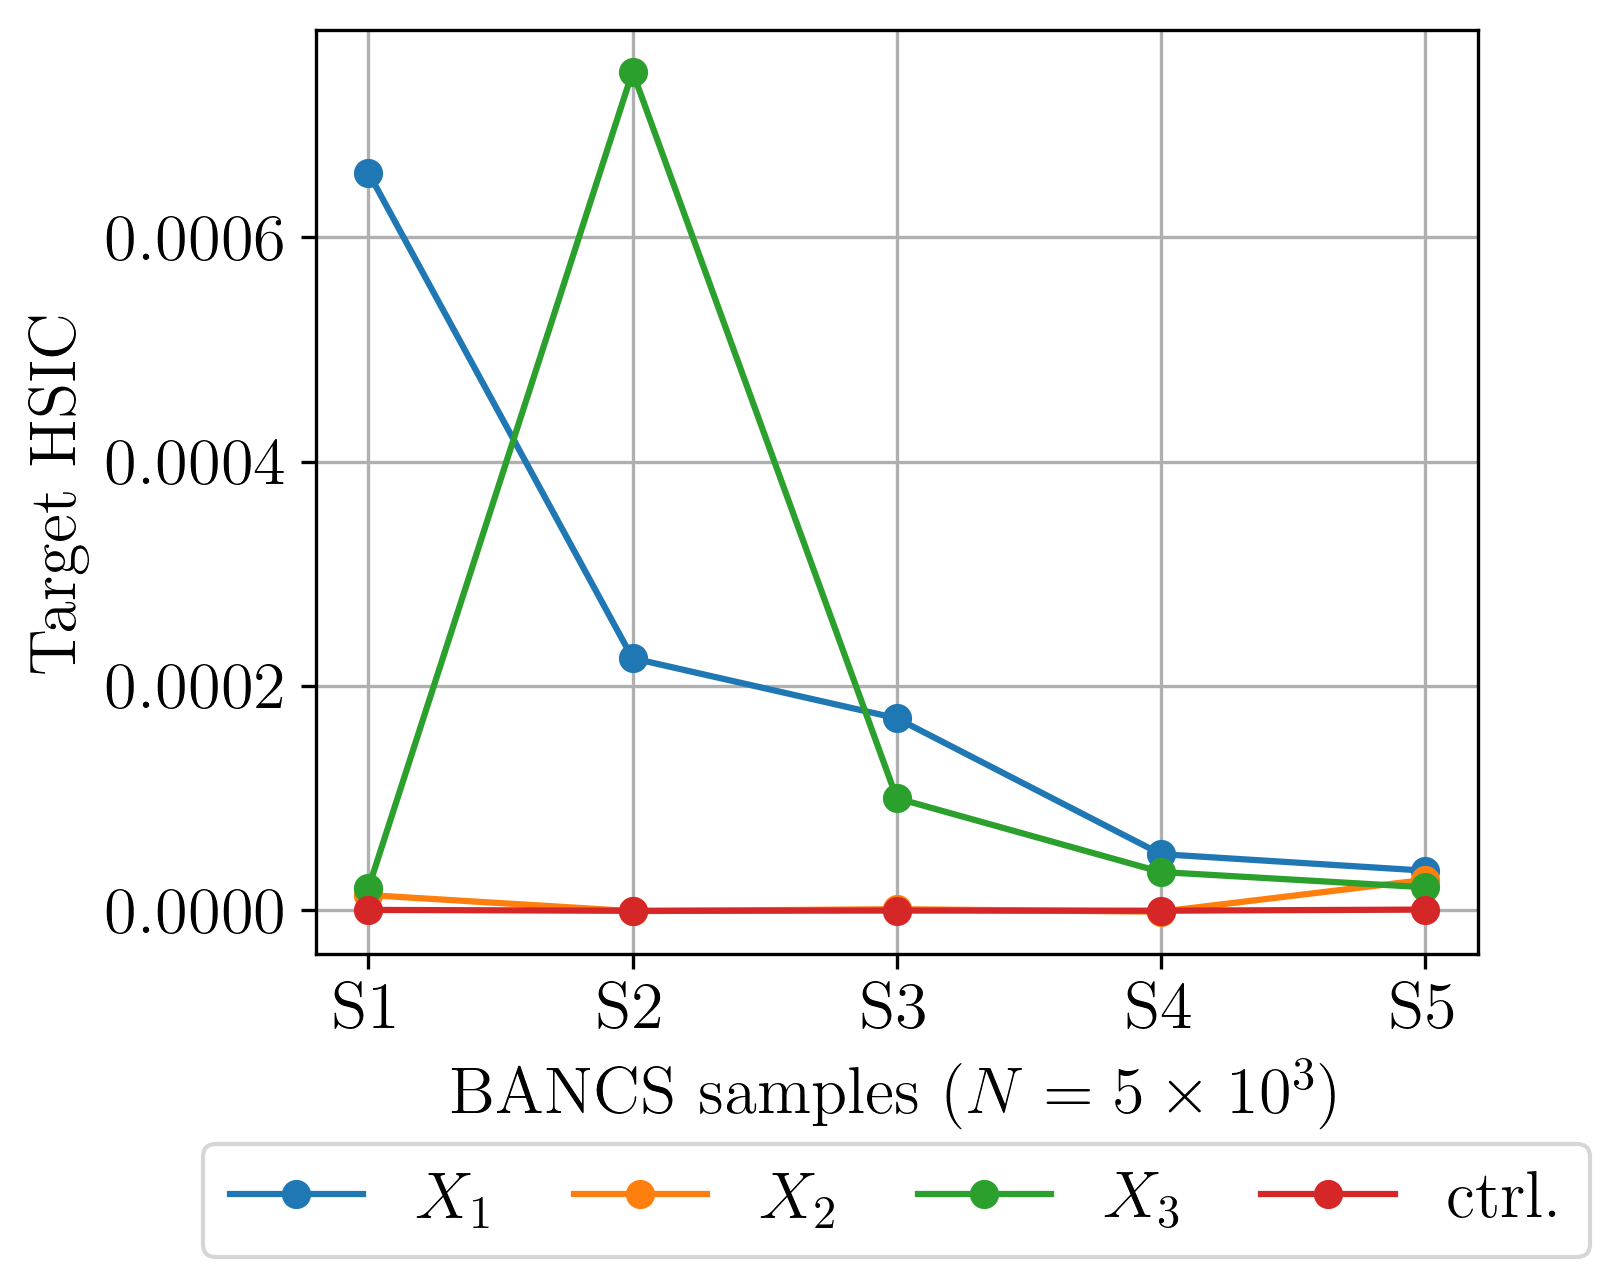
\includegraphics[width=\linewidth]{part3/figures/BANCS/ishigami_THSIC.png}
        \caption{Target $\HSIC(X_j, Y)$.}
    \end{subfigure}
    \begin{subfigure}[b]{0.48\linewidth}
        \centering
        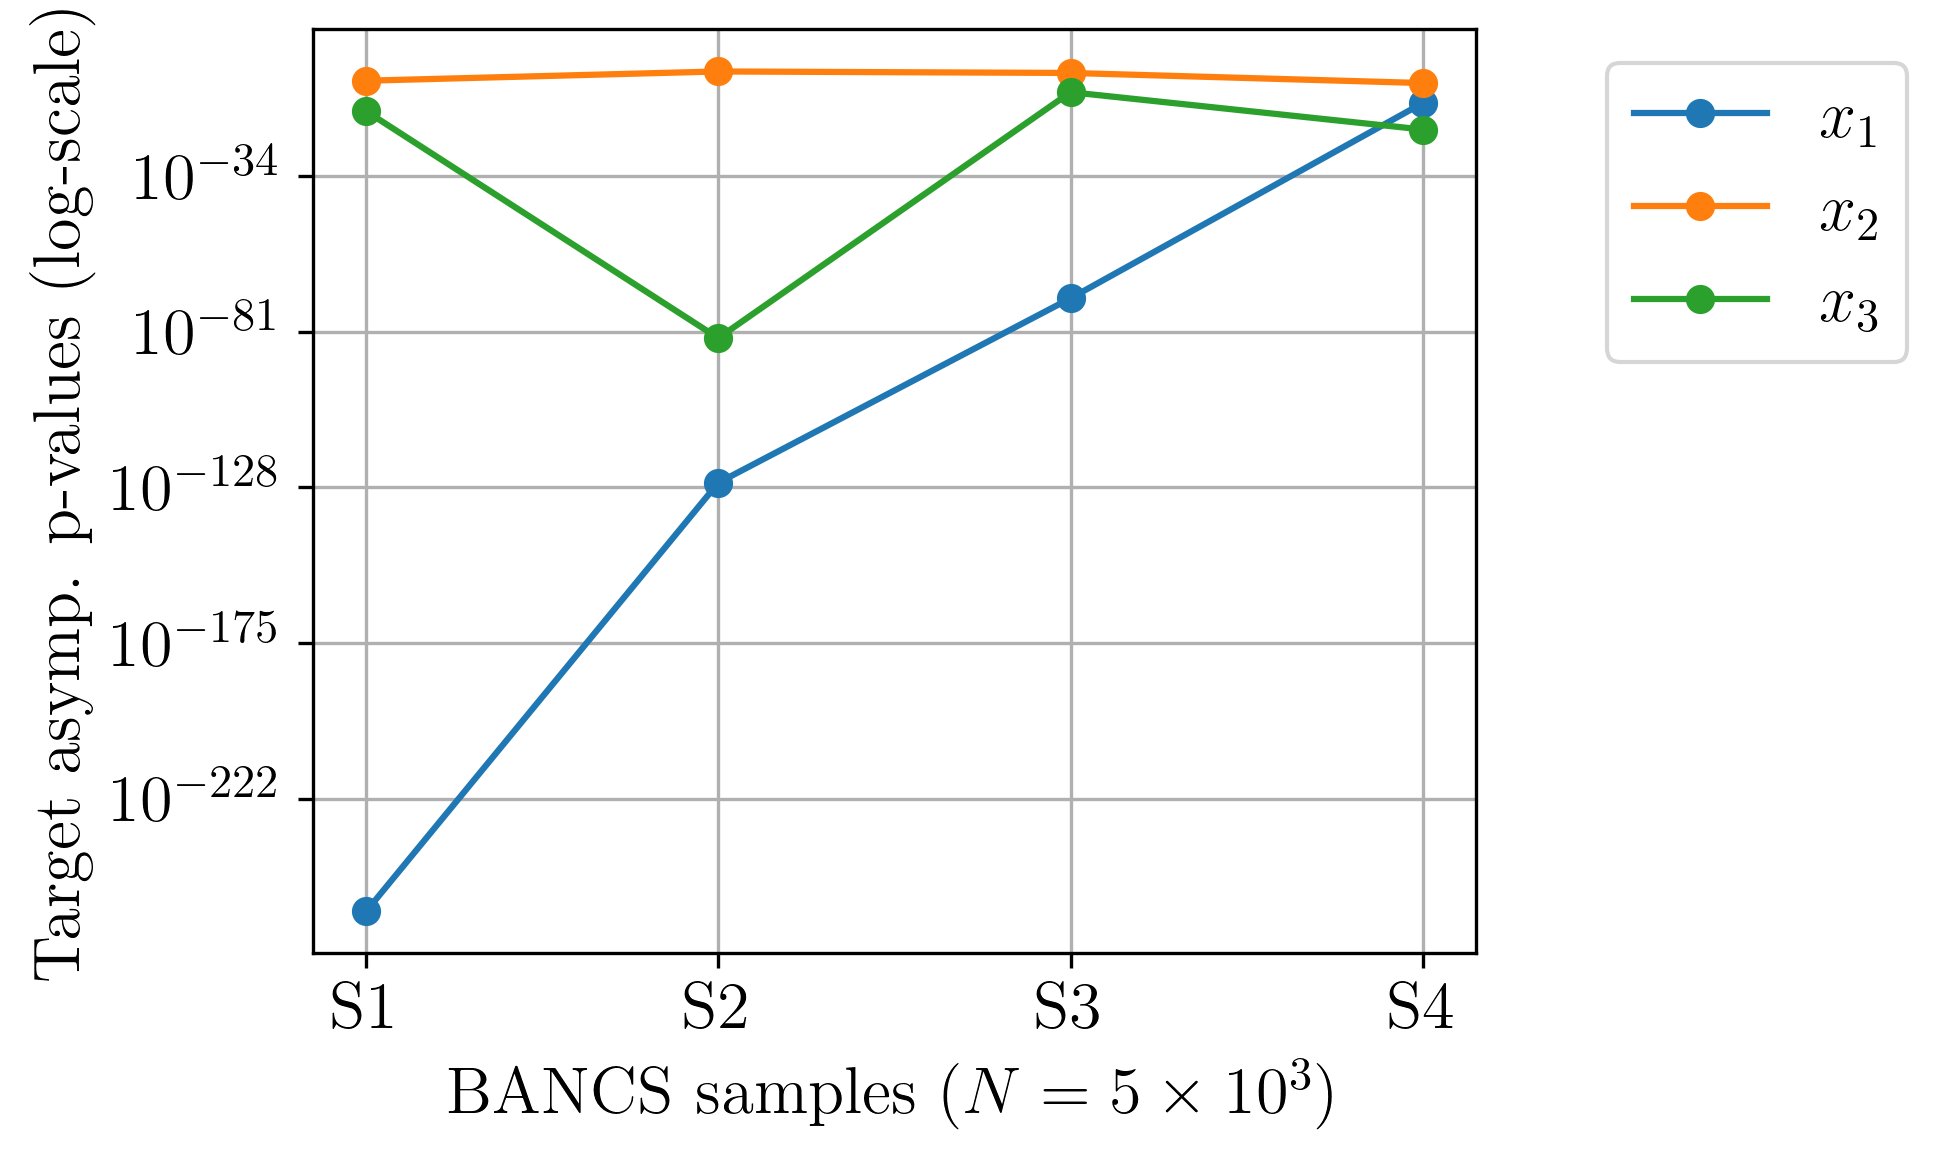
\includegraphics[width=\linewidth]{part3/figures/BANCS/ishigami_Tpvalue_asymptotic.png}
        \caption{Target asymptotic p-values.}
    \end{subfigure}
    \\[20pt]
    \begin{subfigure}[b]{0.48\linewidth}
        \centering
        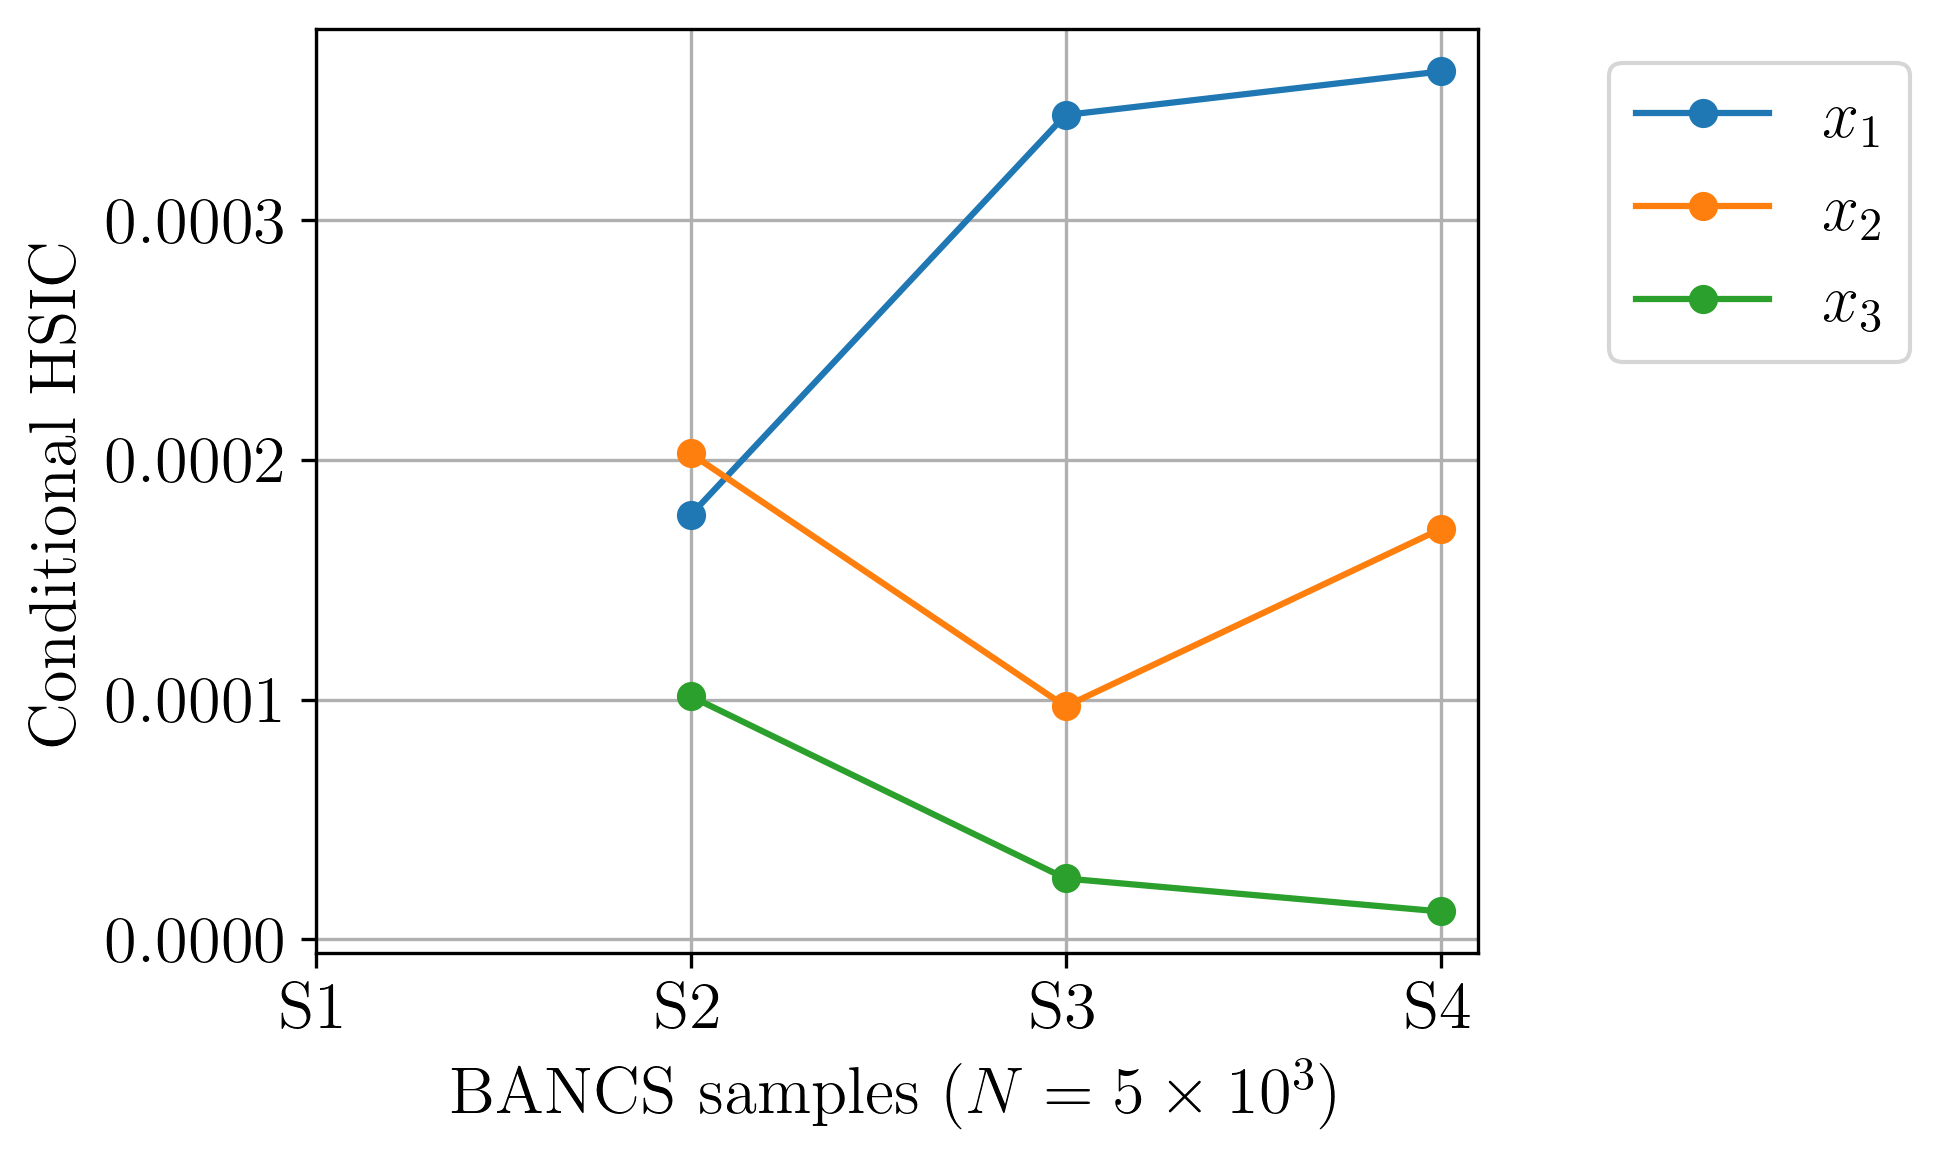
\includegraphics[width=\linewidth]{part3/figures/BANCS/ishigami_CHSIC.png}
        \caption{Conditional $\HSIC(X_j, Y)$.}
    \end{subfigure}
    \begin{subfigure}[b]{0.48\linewidth}
        \centering
        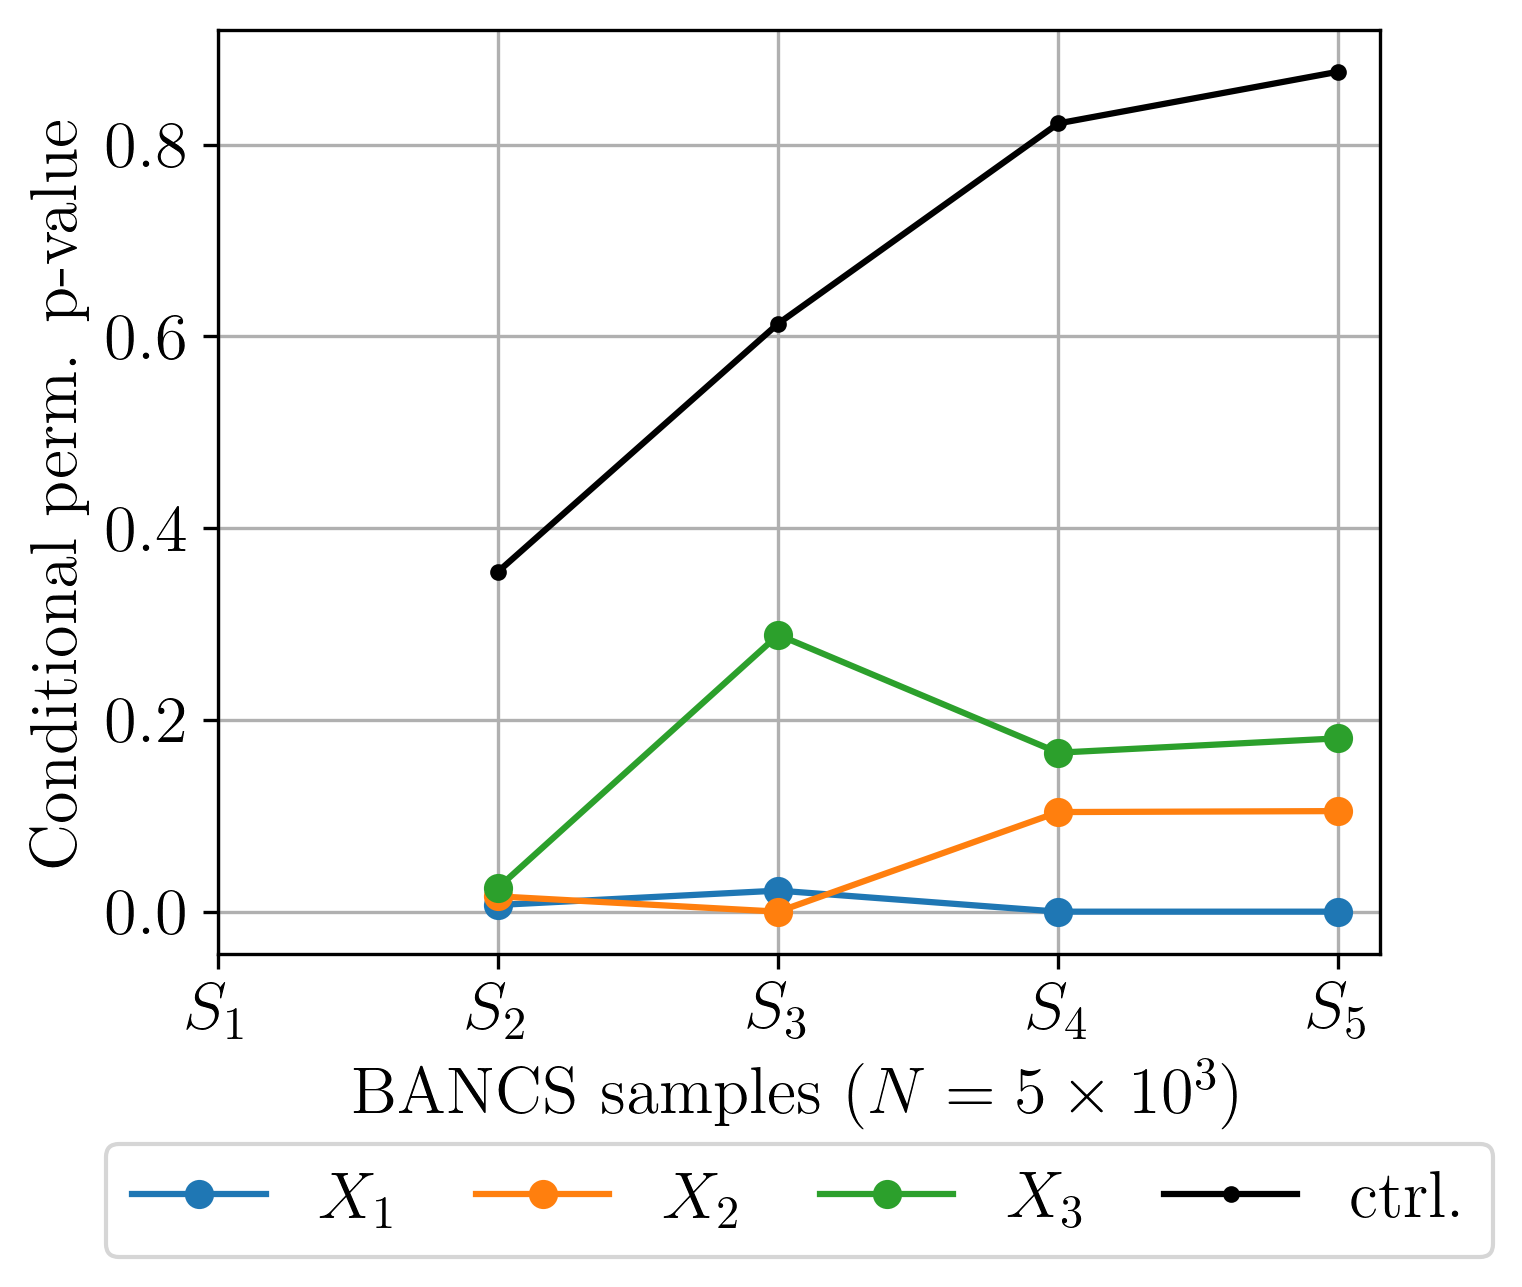
\includegraphics[width=\linewidth]{part3/figures/BANCS/ishigami_Cpvalue_permutation.png}
        \caption{Conditional p-values by perm. ($10^3$ perm.).}
    \end{subfigure}
    \caption{Target and conditional HSIC indices and p-values as a post-processing of a reliability analysis by BANCS for the test case \#3 (modified Ishigami). 
                The consecutive samples from BANCS are denoted by $\{S_k\}_{k=1}^{k_\#}$ (each with size $N=5\times10^3$, with $p_0=0.25$).}
    \label{fig:rosa_ishigami}
\end{figure}


\begin{figure}
    \centering
    \begin{subfigure}[b]{0.48\linewidth}
        \centering
        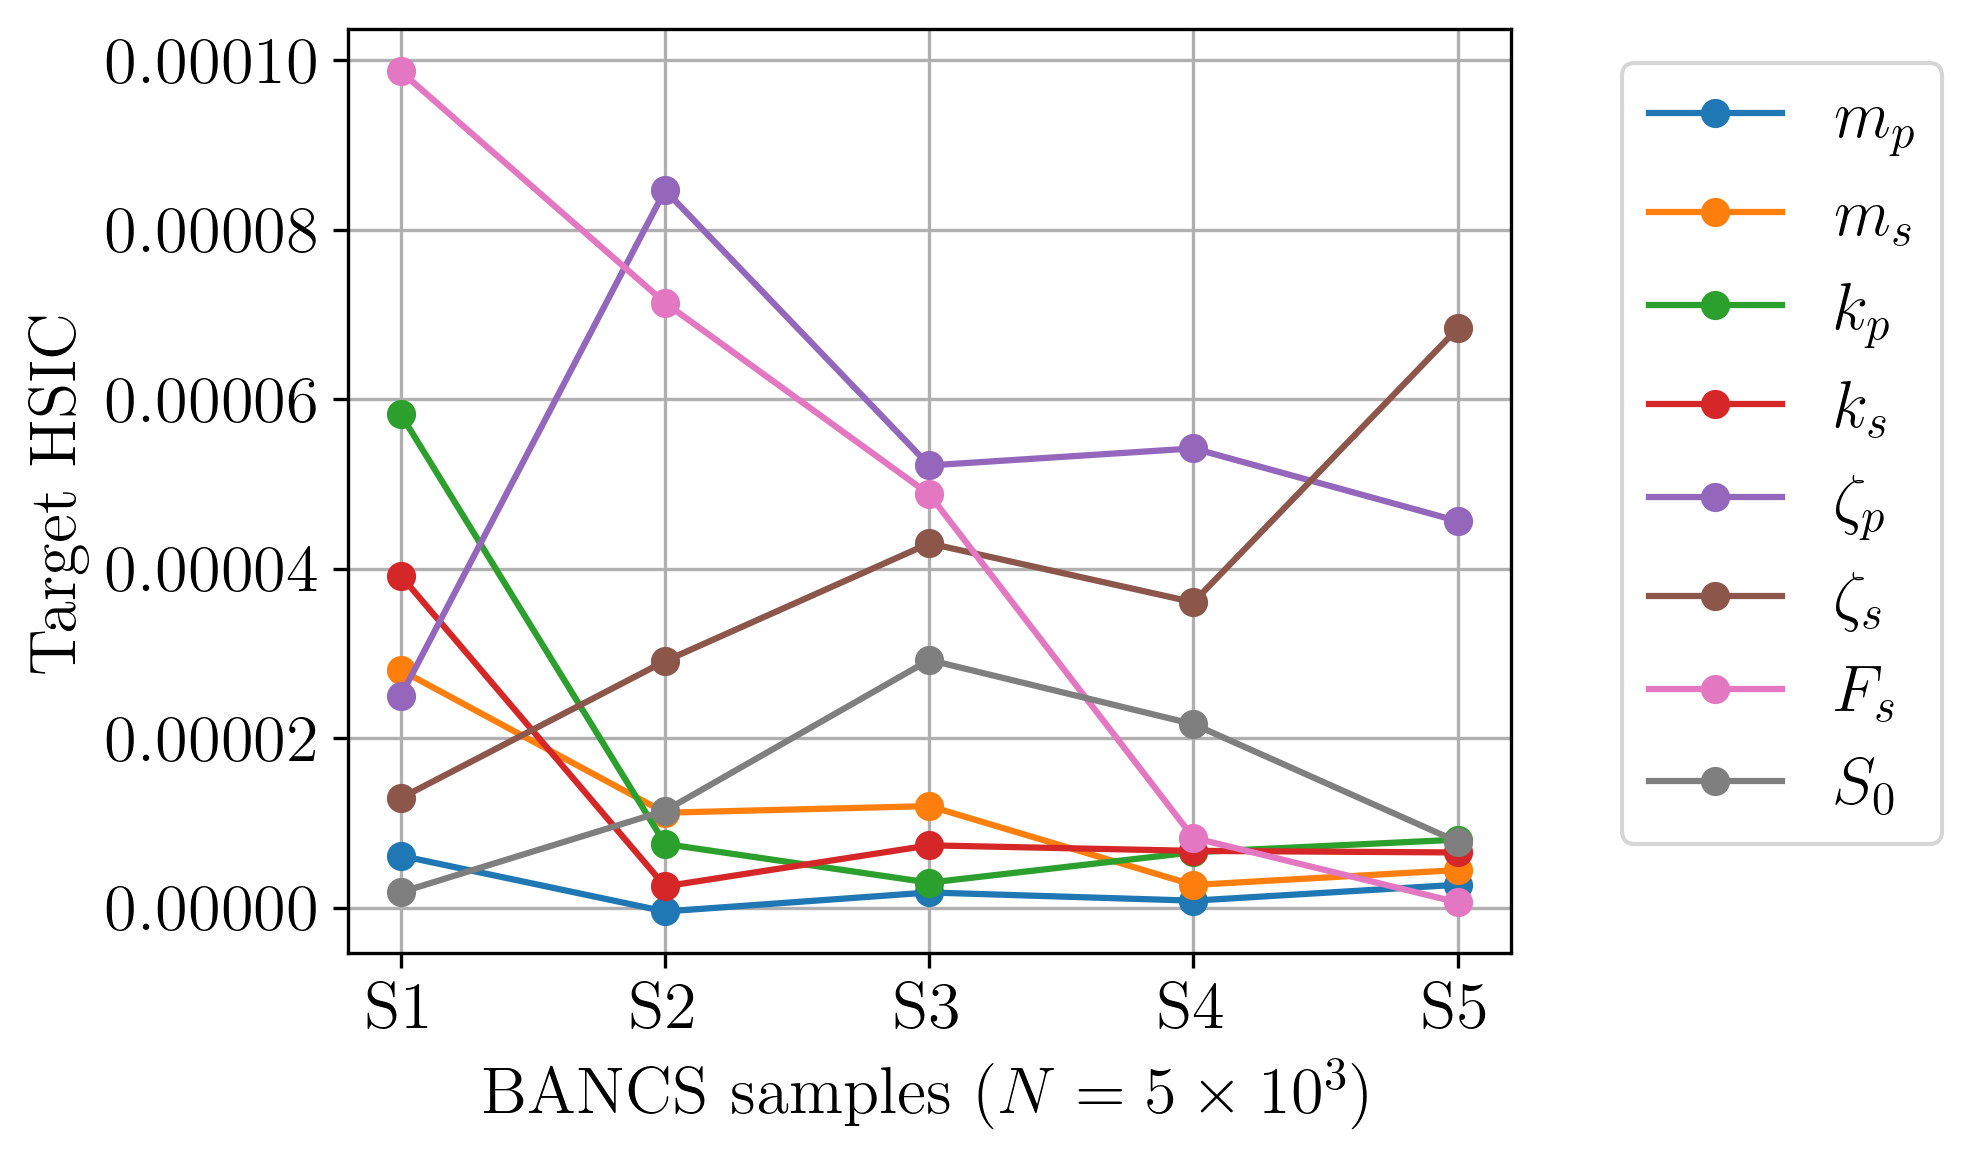
\includegraphics[width=\linewidth]{part3/figures/BANCS/oscillator_THSIC.png}
        \caption{Target $\HSIC(X_j, Y)$.}
    \end{subfigure}
    \hfill
    \begin{subfigure}[b]{0.48\linewidth}
        \centering
        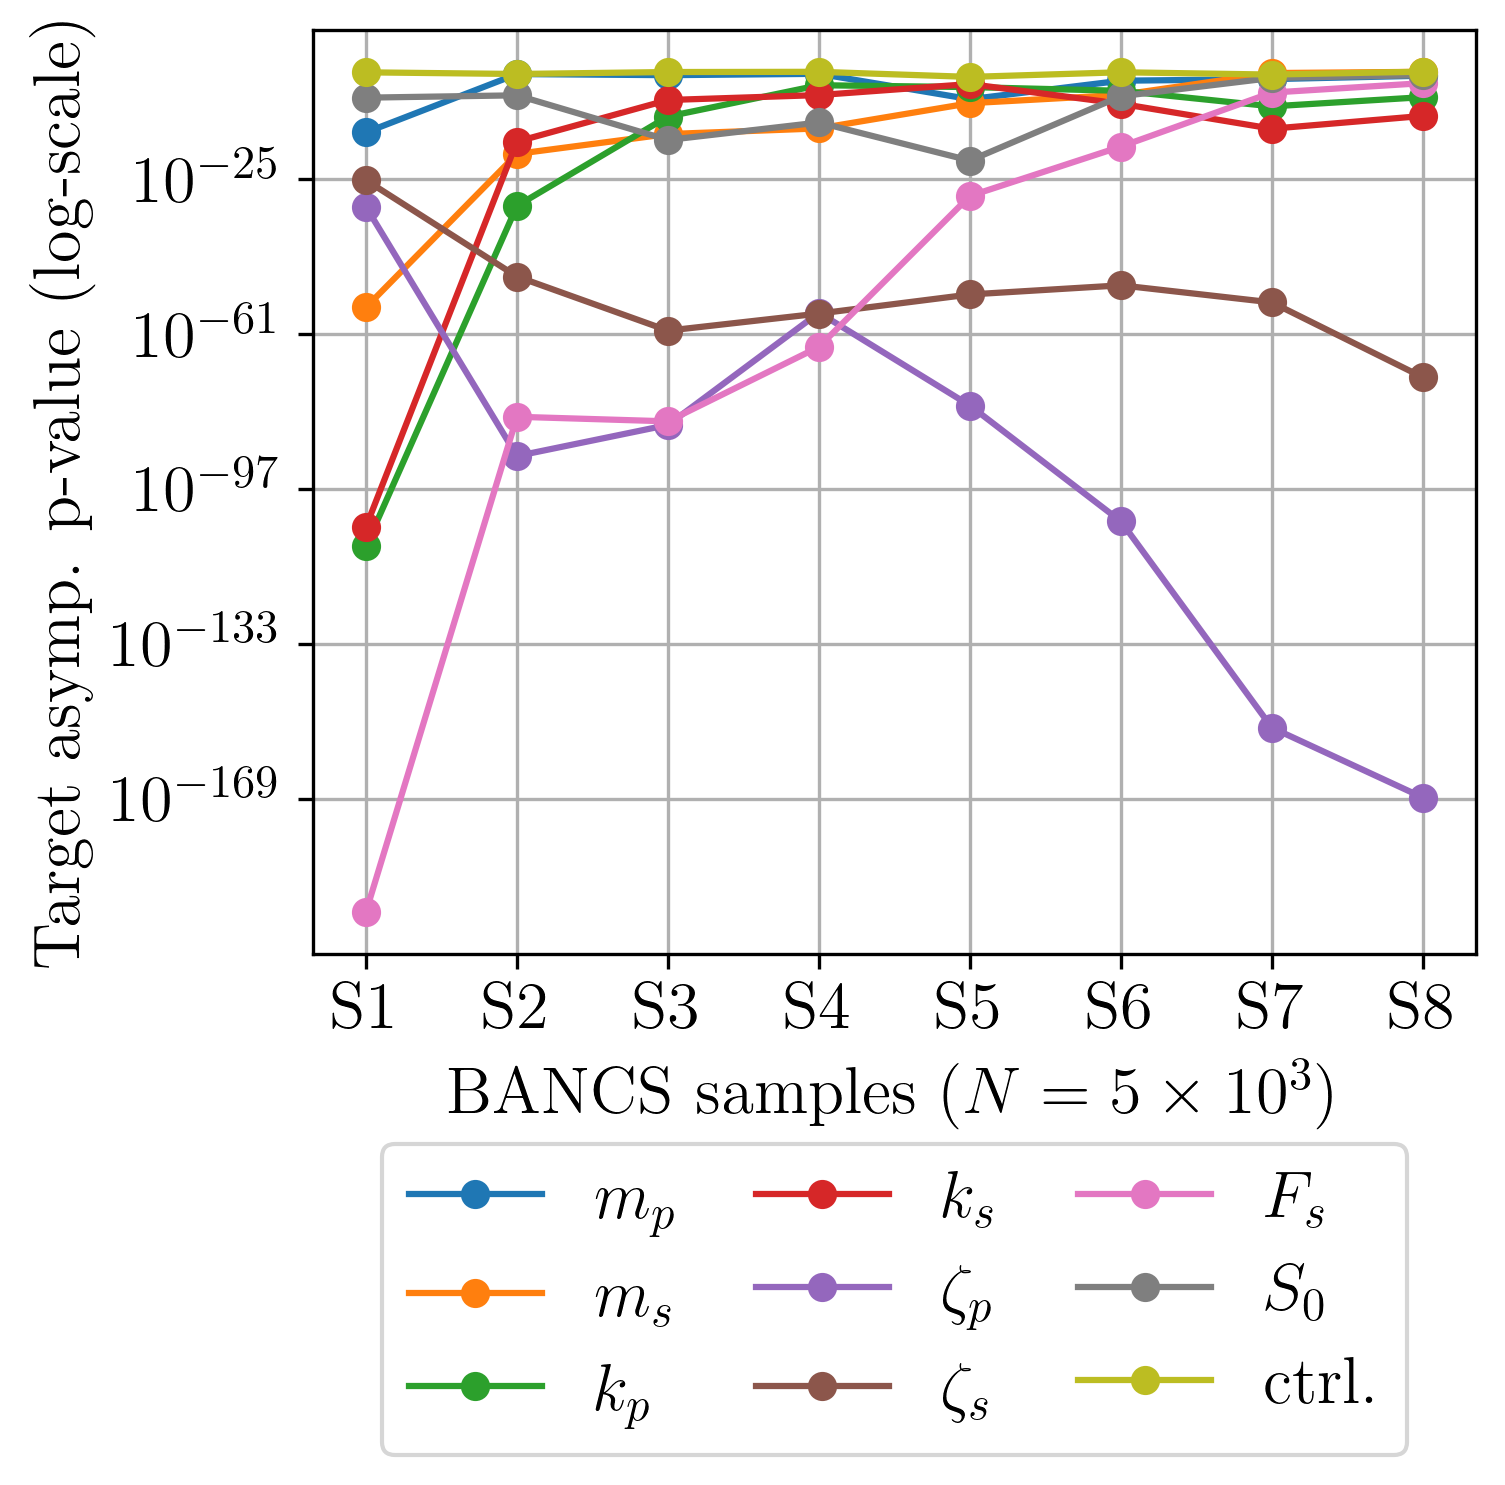
\includegraphics[width=\linewidth]{part3/figures/BANCS/oscillator_Tpvalue_asymptotic.png}
        \caption{Target asymptotic p-values.}
    \end{subfigure}
    \\[20pt]
    \begin{subfigure}[b]{0.48\linewidth}
        \centering
        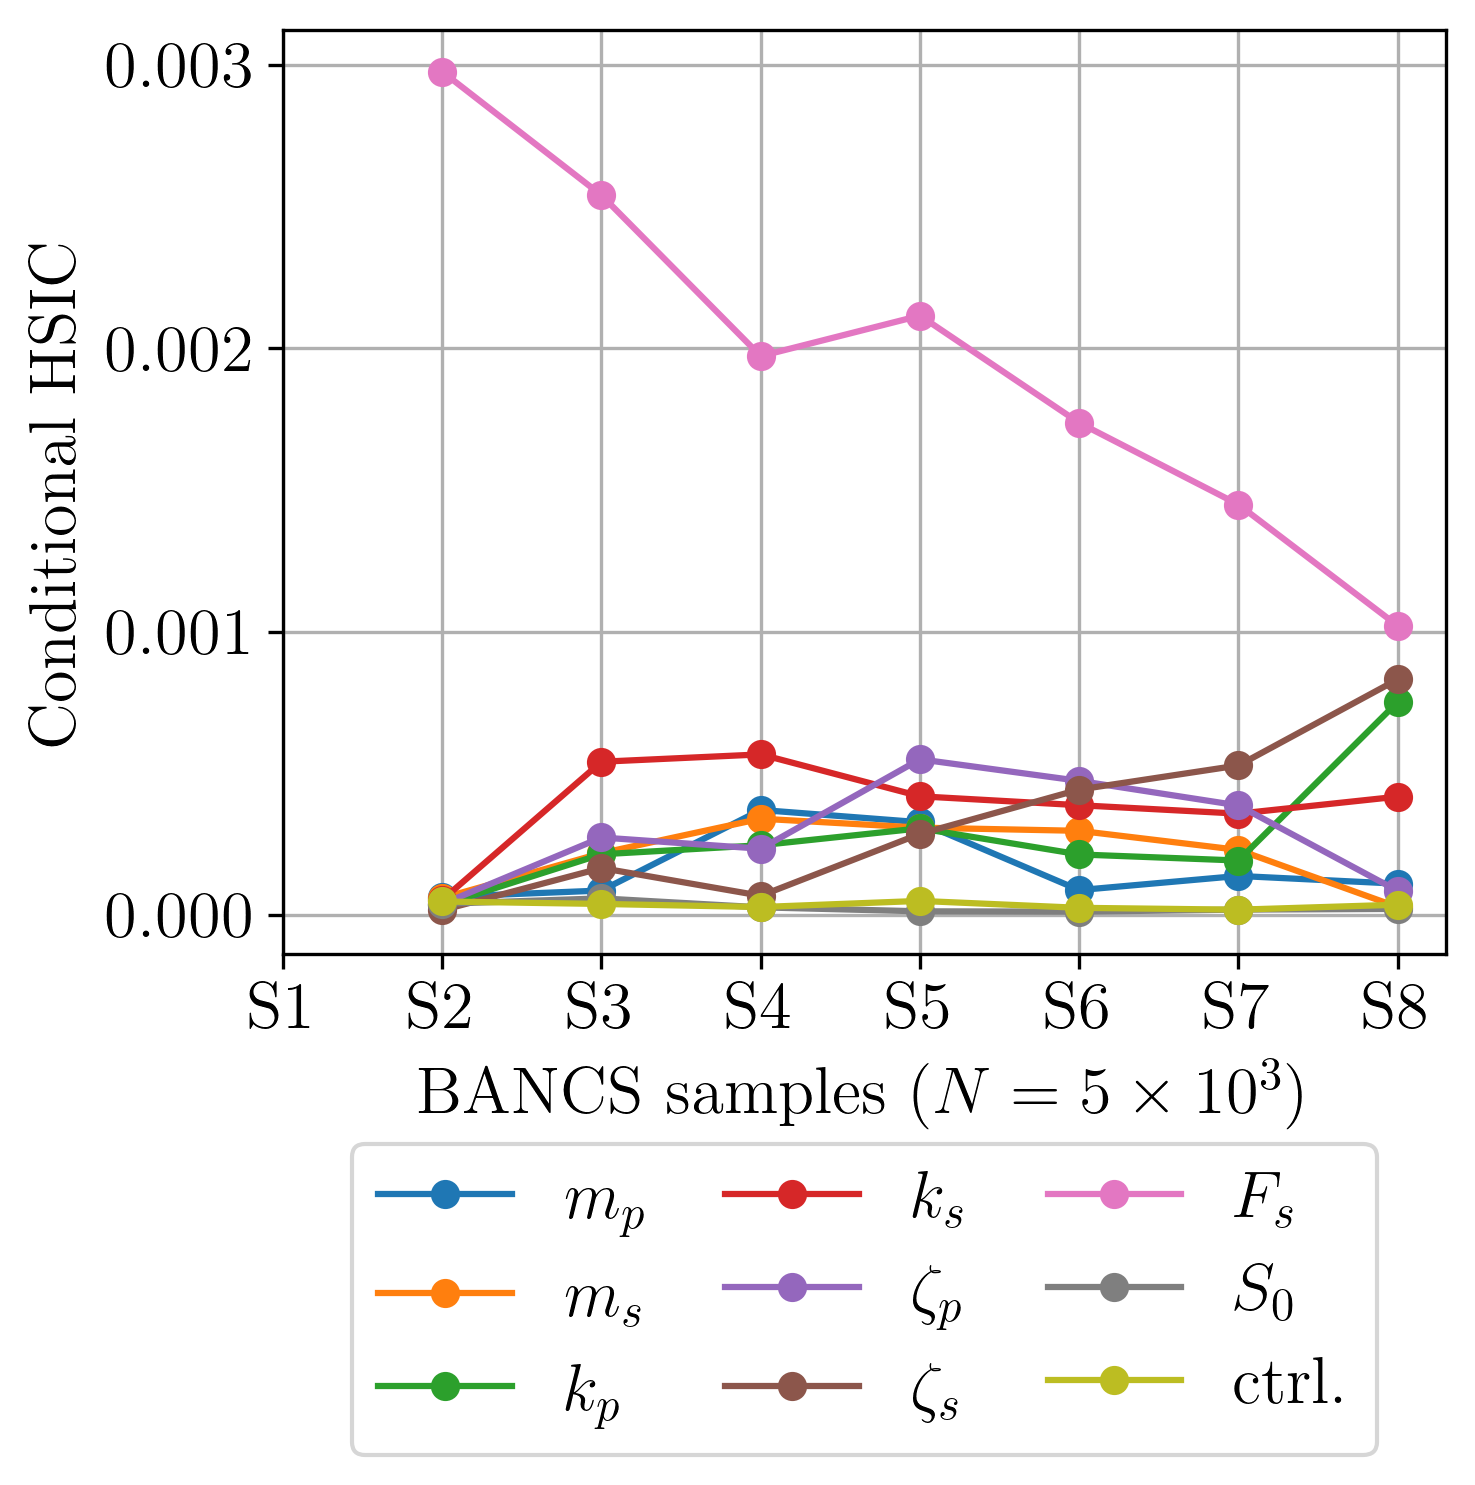
\includegraphics[width=\linewidth]{part3/figures/BANCS/oscillator_CHSIC.png}
        \caption{Conditional $\HSIC(X_j, Y)$.}
    \end{subfigure}
    \hfill
    \begin{subfigure}[b]{0.48\linewidth}
        \centering
        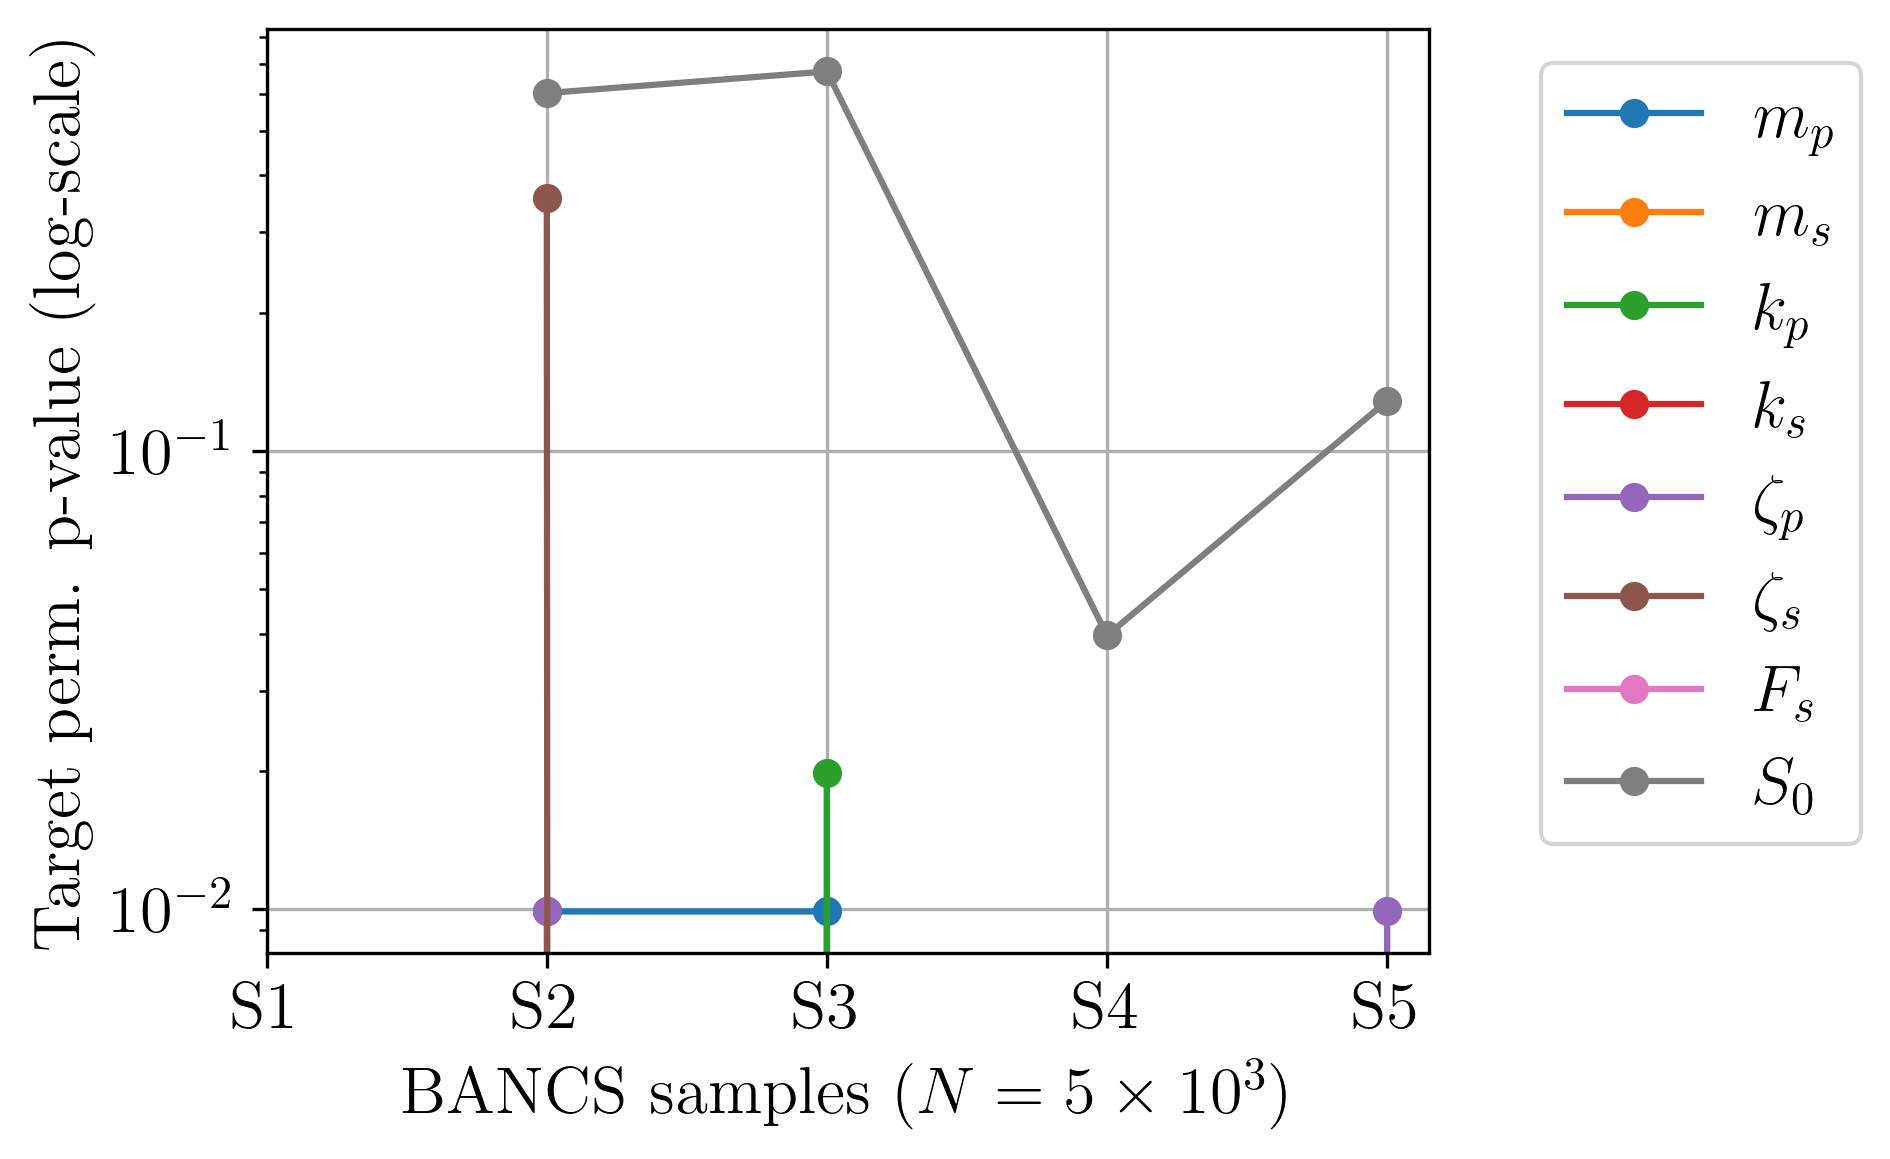
\includegraphics[width=\linewidth]{part3/figures/BANCS/oscillator_Cpvalue_permutation.png}
        \caption{Conditional p-values by perm. ($10^3$ perm.).}
    \end{subfigure}
    \caption{Target and conditional HSIC indices and p-values as a post-processing of a reliability analysis by BANCS for the test case \#5 (nonlinear oscillator problem). 
    The consecutive samples from BANCS are denoted by $\{S_k\}_{k=1}^{k_\#}$ (each with size $N=5\times10^3$, with $p_0=0.25$).}
    \label{fig:rosa_oscillator}
\end{figure}


\begin{figure}
    \centering
    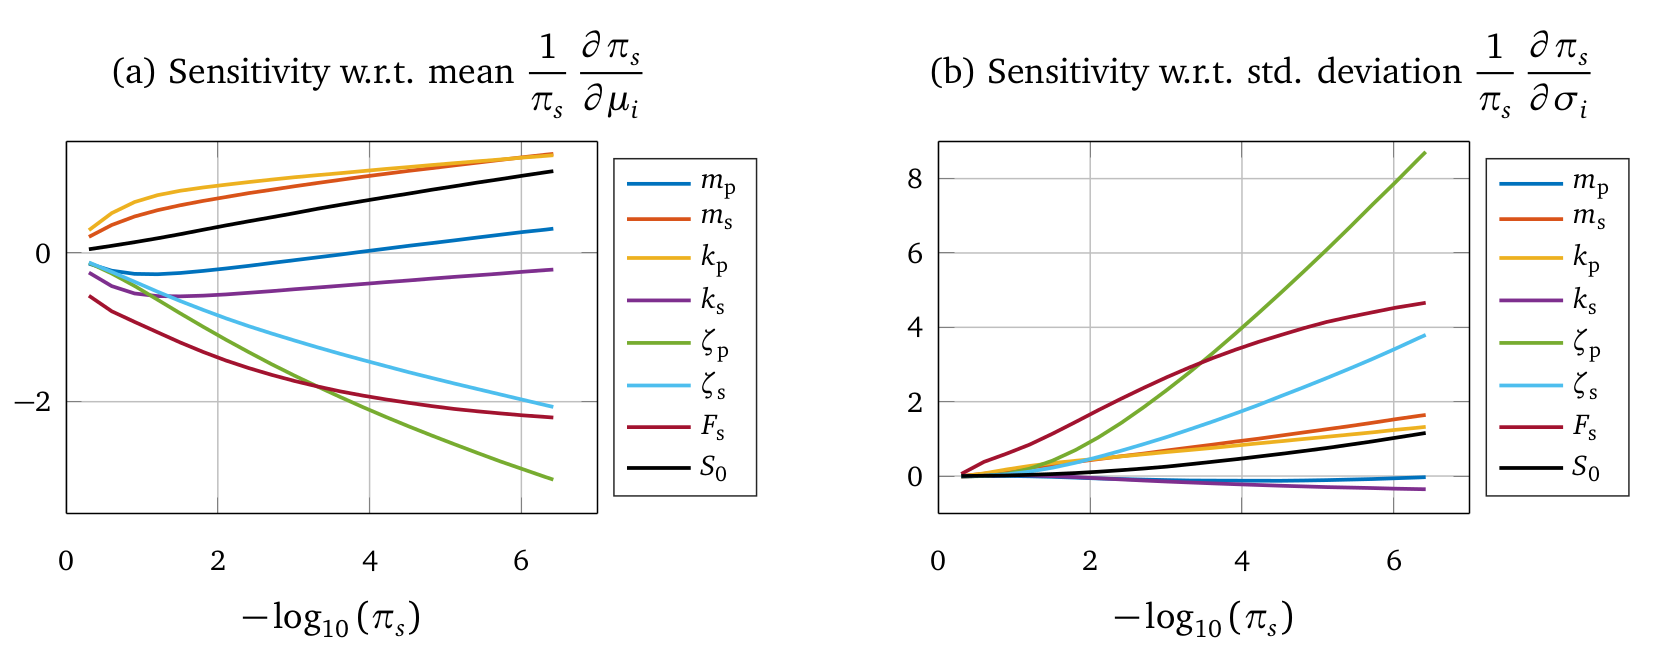
\includegraphics[width=0.9\linewidth]{part3/figures/BANCS/score_function_HDR_JMB.png}
    \caption{Normalized score-functions of $\pi_s = \Pi_{k=1}^s p_0$ w.r.t. the inputs mean $\mu_i$ and standard deviation $\sigma_i$ in the standard normal space (source: \citealp[p.54]{bourinet_2018}). 
            The consecutive probabilities result from a SS (with $N=10^6$ and $p_0=0.5$ per subset).}
    \label{fig:score_functions_oscillator}
\end{figure}



%============================================================%
%============================================================%
\section{Conclusion}
%============================================================%
%============================================================%

In this chapter a contribution to rare event estimation was presented. 
BANCS is a new adaptive importance sampling method using EBC to fit the successive conditional distributions. 
Its performance was compared in a numerical benchmark with other methods such as SS and NAIS. 
The current implementation is at least as efficient as the other methods on the analytical problems studied while generating i.i.d. samples that can be reused for ROSA. 
However, numerous potential improvement remain unexplored. 
A first perspective lies in the optimization of the EBC polynomial order by applying a validation procedure similar to what is done for surrogate models (among the elite set, a test set could be selected using the results from Chapter~\ref{chpt:5}). 
Then, instead of estimating the intermediary quantiles by Monte Carlo, other sampling methods could be tested (e.g., LHS, randomized QMC, see \citealp{tuffin_2019}). 
To tackle high-dimentional problems, the inference of copulas by blocks could be interesting (see e.g., \citealp{lasserre_2022}).

BANCS also presents multiple advantages, first, it does not require a transformation in the standard space, second, its flexibility allows to capture multimodal problems. 
A third advantage is that the samples generated at each iteration are i.i.d., offering the possibility to estimate ROSA indices as a post-processing. 
In this chapter, ROSA was investigated using the HSIC (following the work of \citealp{marrel_chabridon_2021}) but the use of target Shapley effects \citep{ilidrissi_2021_rosa} could also provide an interesting insight for problems with dependent inputs.
Additionally, the recently developed HSIC-ANOVA indices \citep{daveiga_2021_kernel_ANOVA,sarazin_2023} could be explored to capture influences due to complex interactions between variables.
This complementary ROSA is essential to understand the influence of the inputs on the failure probability. 
Further studies should be conducted on how to use these indices for high-dimensional screening in reliability assessment.


%\begin{itemize}
%    \item Compare the learning-time with NAIS
%    \item Perspective learning the entire distribution with Bernstein polynomials
%    \item learning the copula by blocks to tackle high-dimensional problems
%    \item Estimate the quantiles with IS on all previous samples
%    
%    \item Advantage of working directly in the physical space directly
%    \item We could fit the marginals with parametric models and compare
%\end{itemize}
